%%% The main file. It contains definitions of basic parameters and includes all other parts.

%% Settings for single-side (simplex) printing
% Margins: left 40mm, right 25mm, top and bottom 25mm
% (but beware, LaTeX adds 1in implicitly)
\documentclass[12pt,a4paper]{report}
\setlength\textwidth{145mm}
\setlength\textheight{247mm}
\setlength\oddsidemargin{15mm}
\setlength\evensidemargin{15mm}
\setlength\topmargin{0mm}
\setlength\headsep{0mm}
\setlength\headheight{0mm}
% \openright makes the following text appear on a right-hand page
\let\openright=\clearpage

%% Settings for two-sided (duplex) printing
% \documentclass[12pt,a4paper,twoside,openright]{report}
% \setlength\textwidth{145mm}
% \setlength\textheight{247mm}
% \setlength\oddsidemargin{14.2mm}
% \setlength\evensidemargin{0mm}
% \setlength\topmargin{0mm}
% \setlength\headsep{0mm}
% \setlength\headheight{0mm}
% \let\openright=\cleardoublepage

%% Generate PDF/A-2u
\usepackage[a-2u]{pdfx}

%% Character encoding: usually latin2, cp1250 or utf8:
\usepackage[utf8]{inputenc}

%% Prefer Latin Modern fonts
\usepackage{lmodern}

%% Further useful packages (included in most LaTeX distributions)
\usepackage{amsmath}        % extensions for typesetting of math
\usepackage{amsfonts}       % math fonts
\usepackage{amsthm}         % theorems, definitions, etc.
\usepackage{bbding}         % various symbols (squares, asterisks, scissors, ...)
\usepackage{bm}             % boldface symbols (\bm)
\usepackage{graphicx}       % embedding of pictures
\usepackage{fancyvrb}       % improved verbatim environment
\usepackage{natbib}         % citation style AUTHOR (YEAR), or AUTHOR [NUMBER]
\usepackage[nottoc]{tocbibind} % makes sure that bibliography and the lists
			    % of figures/tables are included in the table
			    % of contents
\usepackage{dcolumn}        % improved alignment of table columns
\usepackage{booktabs}       % improved horizontal lines in tables
\usepackage{paralist}       % improved enumerate and itemize
\usepackage{xcolor}         % typesetting in color
\usepackage{soulutf8}			% highlighting text

% -----
% just some workarounds for soul to cooperate with xcolor
% taken from https://tex.stackexchange.com/questions/48501/soul-broken-highlighting-with-xcolor-when-using-selectcolormodel
\usepackage{etoolbox}
\makeatletter
\patchcmd{\SOUL@ulunderline}{\dimen@}{\SOUL@dimen}{}{}
\patchcmd{\SOUL@ulunderline}{\dimen@}{\SOUL@dimen}{}{}
\patchcmd{\SOUL@ulunderline}{\dimen@}{\SOUL@dimen}{}{}
\newdimen\SOUL@dimen
\makeatother
% -----

\usepackage{tikz}
\usepackage{subcaption}
\usepackage[linesnumbered,vlined,ruled]{algorithm2e}    % pseudo - codes
\usepackage{listings} % python code in latex
\usetikzlibrary{positioning}

% declaring argmin
\DeclareMathOperator*{\argmax}{arg\,max}

%%% Basic information on the thesis

% Thesis title in English (exactly as in the formal assignment)
\def\ThesisTitle{Generating text from structured data}

% Author of the thesis
\def\ThesisAuthor{František Trebuňa}

% Year when the thesis is submitted
\def\YearSubmitted{2021}

% Name of the department or institute, where the work was officially assigned
% (according to the Organizational Structure of MFF UK in English,
% or a full name of a department outside MFF)
\def\Department{Institute of Formal and Applied Linguistics (ÚFAL)}

% Is it a department (katedra), or an institute (ústav)?
\def\DeptType{Institute}

% Thesis supervisor: name, surname and titles
\def\Supervisor{Mgr. Rudolf Rosa, Ph.D.}

% Supervisor's department (again according to Organizational structure of MFF)
\def\SupervisorsDepartment{Institute of Formal and Applied Linguistics (ÚFAL)}

% Study programme and specialization
\def\StudyProgramme{Computer Science (B1801)}
\def\StudyBranch{General Computer Science Bc. R9 (NIOI9B)}

% An optional dedication: you can thank whomever you wish (your supervisor,
% consultant, a person who lent the software, etc.)
\def\Dedication{%
Dedication.
}

% Abstract (recommended length around 80-200 words; this is not a copy of your thesis assignment!)
\def\Abstract{%
Abstract.
}

% 3 to 5 keywords (recommended), each enclosed in curly braces
\def\Keywords{%
{text generation} {structured data} {natural language processing} {neural networks}
}

%% The hyperref package for clickable links in PDF and also for storing
%% metadata to PDF (including the table of contents).
%% Most settings are pre-set by the pdfx package.
\hypersetup{unicode}
\hypersetup{breaklinks=true}

% Definitions of macros (see description inside)
%%% This file contains definitions of various useful macros and environments %%%
%%% Please add more macros here instead of cluttering other files with them. %%%

%%% Minor tweaks of style

% These macros employ a little dirty trick to convince LaTeX to typeset
% chapter headings sanely, without lots of empty space above them.
% Feel free to ignore.
\makeatletter
\def\@makechapterhead#1{
  {\parindent \z@ \raggedright \normalfont
   \Huge\bfseries \thechapter. #1
   \par\nobreak
   \vskip 20\p@
}}
\def\@makeschapterhead#1{
  {\parindent \z@ \raggedright \normalfont
   \Huge\bfseries #1
   \par\nobreak
   \vskip 20\p@
}}
\makeatother

% This macro defines a chapter, which is not numbered, but is included
% in the table of contents.
\def\chapwithtoc#1{
\chapter*{#1}
\addcontentsline{toc}{chapter}{#1}
}

% Draw black "slugs" whenever a line overflows, so that we can spot it easily.
\overfullrule=1mm

%%% Macros for definitions, theorems, claims, examples, ... (requires amsthm package)

\theoremstyle{plain}
\newtheorem{thm}{Theorem}
\newtheorem{lemma}[thm]{Lemma}
\newtheorem{claim}[thm]{Claim}

\theoremstyle{plain}
\newtheorem{defn}{Definition}

\theoremstyle{remark}
\newtheorem*{cor}{Corollary}
\newtheorem*{rem}{Remark}
\newtheorem*{example}{Example}

%%% An environment for proofs

\newenvironment{myproof}{
  \par\medskip\noindent
  \textit{Proof}.
}{
\newline
\rightline{$\qedsymbol$}
}

%%% An environment for typesetting of program code and input/output
%%% of programs. (Requires the fancyvrb package -- fancy verbatim.)

\DefineVerbatimEnvironment{code}{Verbatim}{fontsize=\small, frame=single}

%%% The field of all real and natural numbers
\newcommand{\R}{\mathbb{R}}
\newcommand{\N}{\mathbb{N}}

%%% Useful operators for statistics and probability
\DeclareMathOperator{\pr}{\textsf{P}}
\DeclareMathOperator{\E}{\textsf{E}\,}
\DeclareMathOperator{\var}{\textrm{var}}
\DeclareMathOperator{\sd}{\textrm{sd}}

%%% Transposition of a vector/matrix
\newcommand{\T}[1]{#1^\top}

%%% Various math goodies
\newcommand{\goto}{\rightarrow}
\newcommand{\gotop}{\stackrel{P}{\longrightarrow}}
\newcommand{\maon}[1]{o(n^{#1})}
\newcommand{\abs}[1]{\left|{#1}\right|}
\newcommand{\dint}{\int_0^\tau\!\!\int_0^\tau}
\newcommand{\isqr}[1]{\frac{1}{\sqrt{#1}}}

%%% Various table goodies
\newcommand{\pulrad}[1]{\raisebox{1.5ex}[0pt]{#1}}
\newcommand{\mc}[1]{\multicolumn{1}{c}{#1}}


% Title page and various mandatory informational pages
\begin{document}
%%% Title page of the thesis and other mandatory pages

%%% Title page of the thesis

\pagestyle{empty}
\hypersetup{pageanchor=false}
\begin{center}

\centerline{\mbox{\includegraphics[width=166mm]{img/logo-en.pdf}}}

\vspace{-8mm}
\vfill

{\bf\Large BACHELOR THESIS}

\vfill

{\LARGE\ThesisAuthor}

\vspace{15mm}

{\LARGE\bfseries\ThesisTitle}

\vfill

\Department

\vfill

{
\centerline{\vbox{\halign{\hbox to 0.45\hsize{\hfil #}&\hskip 0.5em\parbox[t]{0.45\hsize}{\raggedright #}\cr
Supervisor of the bachelor thesis:&\Supervisor \cr
\noalign{\vspace{2mm}}
Study programme:&\StudyProgramme \cr
\noalign{\vspace{2mm}}
Study branch:&\StudyBranch \cr
}}}}

\vfill

% Zde doplňte rok
Prague \YearSubmitted

\end{center}

\newpage

%%% Here should be a bound sheet included -- a signed copy of the "bachelor
%%% thesis assignment". This assignment is NOT a part of the electronic
%%% version of the thesis. DO NOT SCAN.

%%% A page with a solemn declaration to the bachelor thesis

\openright
\hypersetup{pageanchor=true}
\pagestyle{plain}
\pagenumbering{roman}
\vglue 0pt plus 1fill

\noindent
I declare that I carried out this bachelor thesis independently, and only with the cited
sources, literature and other professional sources. It has not been used to obtain another
or the same degree.

\medskip\noindent
I understand that my work relates to the rights and obligations under the Act No.~121/2000 Sb.,
the Copyright Act, as amended, in particular the fact that the Charles
University has the right to conclude a license agreement on the use of this
work as a school work pursuant to Section 60 subsection 1 of the Copyright~Act.

\vspace{10mm}

\hbox{\hbox to 0.5\hsize{%
In \hbox to 6em{\dotfill} date \hbox to 6em{\dotfill}
\hss}\hbox to 0.5\hsize{\dotfill\quad}}
\smallskip
\hbox{\hbox to 0.5\hsize{}\hbox to 0.5\hsize{\hfil Author's signature\hfil}}

\vspace{20mm}
\newpage

%%% Dedication

\openright

\noindent
\Dedication

\newpage

%%% Mandatory information page of the thesis

\openright

\vbox to 0.5\vsize{
\setlength\parindent{0mm}
\setlength\parskip{5mm}

Title:
\ThesisTitle

Author:
\ThesisAuthor

\DeptType:
\Department

Supervisor:
\Supervisor, \SupervisorsDepartment

Abstract:
\Abstract

Keywords:
\Keywords

\vss}

\newpage

\openright
\pagestyle{plain}
\pagenumbering{arabic}
\setcounter{page}{1}


%%% A page with automatically generated table of contents of the bachelor thesis

\tableofcontents

%%% Each chapter is kept in a separate file
\chapter*{Introduction} \label{IntroductionChapter}
\addcontentsline{toc}{chapter}{Introduction}

The Language Modeling is the task of predicting what word comes next in the actual context. In this thesis we delve into a slightly more complicated task, into the Conditional Language Modeling, where the next generated word does not only depend on the context but also on some external factors.

Specifically, given tables of team and individual statistics (e.g. number of points scored by a team,  number of minutes played by a player etc.) we aim to generate a document-scale text that is coherent (e.g. without contradictions), written in good English, and that contains a lot of factual data based on the input tables. We train multiple Deep Neural Network models on the RotoWire dataset \citep{wiseman2017}. It consists of the statistics of National Basketball Association matches from 2014 - 2017 and the corresponding professionally written summaries from the fantasy sports news site \url{https://www.rotowire.com/basketball/}.

The statistics as well as the manual analysis of the dataset show numerous discrepancies (chapter \ref{chapter:preprocessing_and_statistics_of_the_dataset}). We elaborate on various preprocessing and cleaning methods that should make the learning path of our models easier.

We explore the Encoder-Decoder architecture \citep{sutskever2014sequence} along with many enhancements such as the attention (section \ref{section:attention_mechanism}), the copy attention (section \ref{section:copy_mechanism}), and the content selection and planning (section \ref{section:content_selection_and_planning}).

However this kind of architecture is aimed at processing sequential input while the structured data from the RotoWire dataset is in form of tables. Therefore following \citet{wiseman2017} we show the methods that keep most of the valuable positional information while transforming tabular data into a sequence of records. We also discuss the neural network architectures that learn what kind of information is stored in a particular record (section \ref{subsection:baseline_model_encoder}), and which records are complementary to each other (section \ref{subsection:content_selection}).

We hypothesize that the biggest performance bottleneck of our approach is the complexity of the input tables. Therefore we propose two methods which aim to reduce the complexity.

The quality of generated texts is measured using the BLEU score, and a set of manual metrics (Entity Recall measures how many of the entities mentioned in the gold summaries are also in the generated ones, while Factual Correctness measures how many of the generated numerical facts are grounded on the statistics from the input tabular data). We show that enhancements of the Encoder-Decoder architecture as well as the reduction of complexity of the input tables help the performance of our models.

All the models and preprocessing methods are developed in \emph{python 3.8} and \emph{tensorflow 2.4.1}. However the code is compatible with \emph{python 3.6} and \emph{tensorflow 2.3} (the versions used on Artifical Intelligence Cluster (AIC) where the training was executed).
\chapter{Problem statement}
In september 2020 I read a blog by \citep*{Karpathy2015}. He created a neural network consisting of only one LSTM cell and trained it to predict a character based on all the previous ones. The network was trained on a corpus of all the plays by Shakespeare. During inference the last predicted character was fed as the input to the network and this way it could create a really good looking Shakespeare-like text. Then I began to explore the possibilities of generating a text conditioned on some input parameters. How to construct a network that could be told to generate a sad, happy, or sarcastic sounding text?

\section{Data to text generation}
Known datasets (WIKIBIO, WeatherGov, RoboCup) -> short description, the generated summaries are one-two sentences long. Rotowire -> really long summaries although only a fraction of the number of unique tokens from the WIKIBIO dataset. Only short description of the dataset, the statistics and observations are in the second chapter.

\section{Fantasy sports}
What it is, where it originates, the relation to basic optimisation problems, why NLGenerated summaries could be added value.

\section{My goal}
Fluent text which captures the important statistics from the table
\chapter{Data}

One needs a lot of data if he wants to train his neural network. E.g. \citep{sennrich2016} trains the neural machine translation system on 4.2 million English-German sequence pairs. The Data-to-Text generation task má vyššie nároky na kvalitu datasetu. Potrebujeme, aby boli vstupné dáta štandardizované a aby výstupné texty zodpovedali vstupným dátam. Existuje viacero datasetov, ktoré spĺňajú túto podmienku. V tejto kapitole predstavím datasety WikiBIO a Rotowire.

\section{General description}

\showboxdepth=5
\showboxbreadth=5

Obidva tieto datasety používajú notáciu, ktorá bola predstavená v článku od \citep{liang-etal-2009-learning}, preto ju najprv aj tu zadefinujeme.

Ako vstup používame postupnosť záznamov (recordov) $ \mathbf{s} = \{ r_i \}_{i=1}^{J} $. Každý record $ r $ má svoj typ $ r.t \in \mathcal{T} $. Množina typov $\mathcal{T}$ je dopredu definovaná. Ďalej má typ, množinu hodnôt $ r.v = \{ r.v_1, ... , r.f_m\}$. Napríklad v datasete WeatherGOV: $ r.t == windSpeed $, $ r.v = \{time, min, mean, max, mode\}$. Na základe týchto záznamov následne predpovedáme výstupný text $ \mathbf{w} = \{ w_i\}_{i=1}^{ | \mathbf{w} | }$

\section{WikiBIO dataset}

Štruktúrované dáta vo WikiBIO datasete sú vo forme tabuliek. Encoder-Decoder architektúra však vyžaduje, aby do nej boli dáta vkladané sekvenčne. [potrebujem tu pridať príklad tabuľky, pomocou obrázka]. Preto po vzore \citep{lebret2016neural} je tabuľka sploštená do série recordov.Typy sú anotácie riadkov, napríklad meno, dátum narodenia. Príslušných hodnôt však môže byť variabilne veľa. Preto musia vytvorené recordy reflektovať aj poradie hodnôt, čo dosahujeme tým, že pridáme pozičnú informáciu. Recordy sú teda podávané vo formáte $ name_1 = Frantisek, name_2 = Trebuna, birthplace_1 = Kosice, birthplace_2 = Slovensko \dots$ -- pridať informáciu o odlišných dĺžkach tabuliek -- lepší príklad, než vlastné meno --

\subsection{Statistics of WikiBIO dataset}
o tomto píšem zajtra

\subsection {Preprocessing of WikiBIO dataset}
o tomto píšem zajtra


\section{Rotowire dataset}

Štruktúrované dáta v RotoWire datasete sú taktiež vo forme tabuľky. Väčšina hodnôt je vo forme čísla, ktoré buď predstavuje informáciu o absolútnom počte nejakej hodnoty (e.g. počet bodov, ktoré hráč strelil) alebo o relatívnom (e.g. percento úspešných pokusov z poľa). Zvyšné hodnoty sú mená miest, tímov a hráčov. Neskôr uvediem, ako som za pomoci preprocessingu zariadil, aby nebola potrebná pozičná informácia ani v týchto prípadoch. Na rozdiel od WikiBIO datasetu, kde všetky hodnoty pojednávali o jednej entite, v RotoWire potrebujeme ešte špeciálnu informáciu. Teda je potrebné pridať $ r.e $


\subsection{The statistics of the dataset}
General statistics of the dataset before preprocessing - number of tokens, unique tokens, player names, city names. Why we want to make the number of tokens lower while keeping the ability to have rich vocabulary.

\subsection{Cleaning}
Lorem Ipsum as one of the summaries, the paper doesn't mention if it's used as augmentation of the dataset or if it's a bug - removed. Player initials "C.J. McCollum" in table "CJ McCollum" in text. 

\subsection{Transformations of player names, city names and \linebreak[4] team names}
The motivation - making data denser. In a lot of summaries the player is firstly introduced "It was up to LeBron James to take over for Cleveland" and then referenced only by his surname "James finished with 27 points, 14 assists and 8 rebounds..." Many transformations were ommitted although possible. The text looks more natural if the network learns that Philladelphia is sometimes mentioned as Philly. Those nuances are left in the text.

\subsection{Other transformations made to the dataset}
Here I'll mention lowercasing, number transformations.

\subsection{Byte pair encoding}
What it is, who introduced it. How it decreases the number of tokens.

\subsection{The statistics of the transformed dataset}
What is achieved with the use of all the mentioned transformations. The number of unique tokens decreased almost than 4 times (11 300 to 2 900). The fraction of tokens mentioned more than 5 times increased from 47\% to 89,5\%. Highlight the differences to processing of  
\chapter{Preprocessing and Statistics of the Dataset} \label{chapPreproc}

To generate text from structured data I choose the Deep Neural Networks and specifically the Encoder-Decoder (ED) neural architecture (section \ref{neural_nets_chapter}). The ED suited to process sequential one dimensional data, however we cope with two dimensional tables. In this chapter I present the statistics of the dataset \emph{before any preprocessing}. Next I elaborate about the methods of preprocessing and cleaning of the data. In the end I show the statistics of the dataset with all the transformations applied.

\section{Transforming Tables to Records} \label{table_to_record_trans}

At first let's define a table. A table is a two dimensional data structure, where the information is stored not only in the actual values in cells, but also in the positional information. Values in the same column have the same type, whereas values in the same row belong to the same entity. An example of a table as we have defined it is in figure \ref{ex_struct}.

\begin{table}[h]
    \centering
    \begin{tabular}{llll}
        \toprule
        {} & type$_1$ & type$_2$ \dots \\
        \midrule
        entity$_1$ & value$_{1,1}$ &  value$_{1,2}$ \dots \\
        entity$_2$ & value$_{2,1}$ & value$_{2,2}$ \dots \\
        \dots &&
    \end{tabular}
    \caption{An example of structured data} \label{ex_struct}
\end{table}

I use the same notation as \citep{liang-etal-2009-learning}. Table $\mathcal{T}$ is transformed into a sequence of records $ \mathbf{s} = \{ r_i \}_{i=1}^{J} $, where $r_i$ denotes i-th record. To fulfill our goal of keeping the most of the positional information from the table, each record contains field $r.type$ denoting the type of the value, the actual value $r.value$ and the entity $r.entity$ to which the record belongs. At the end, I transform table \ref{ex_struct} to sequence of records \ref{ex_seq_rec}.

\tikzstyle{example_style} = [rectangle, rounded corners, minimum width=3cm, minimum height=1cm,text centered, fill=yellow!10, align=left]

\begin{figure}[!h]
    \centering
    \usetikzlibrary{shapes.multipart}
    \begin{tikzpicture}
    \node (r1) [example_style] {
        \{\emph{type}: type$_1$; \emph{entity}: entity$_1$, \emph{value}: value$_{1,1}$\}
    };
    \node (r2) [example_style, below=2mm of r1]{
        \{\emph{type}: type$_2$; \emph{entity}: entity$_1$, \emph{value}: value$_{1,2}$\}
    };
    \node (r3) [example_style, below=2mm of r2]{
        \{\emph{type}: type$_1$; \emph{entity}: entity$_2$, \emph{value}: value$_{2,1}$\}
    };
    \end{tikzpicture}
    \\ \dots
    \caption{An example of records obtained by transforming table \ref{ex_seq_rec}} \label{ex_seq_rec}
\end{figure}

\section{Dataset Statistics} \label{assumptions_ref}

I believe that the challenges posed by the RotoWire dataset can be summarized in a set of statistics. In this section I want to present the most important ones to help reader to understand the nature of the problem. 

Firstly, the target summaries as well as the sequences of input records are really long compared to other datasets modelling the same task (e.g. WikiBIO \citep{lebret2016neural}, WeatherGOV \citep{liang-etal-2009-learning}, RoboCup \citep{chen2008robocup}).

Secondly, many words occur rarely and the generation system cannot learn a good representation of them (it is known as a \emph{rare word problem}). It should be noted that the problem can be resolved by the means of clever preprocessing (section \ref{bpeSection}) or with help of advanced neural architectures (section \ref{copy_mech_sec}).

Thirdly, there are many values which represent facts, e.g. values that cannot be deduced from the context (e.g. points a player scored in a match etc.) but must be selected and copied from the table.

The original dataset as prepared by \citep{wiseman2017}, is already divided to train (3398 samples), development (727 samples) and test (728 samples) sets. \emph{In the statistics presented below I state that there are only 3397 samples in the train set because one of the samples is the famous Lorem Ipsum template.}

\subsection{Length-wise Statistics}

The input tables contain huge amount of information. 2 teams and up to 30 players participate in a match of basketball. After transformation to a sequence, a player is represented by 24 and a team by 15 records. The type field $r.type$ is the only trait distinguishing the team and player records. Table \ref{stats_tables_orig_rw} summarizes the length statistics of the input sequences. 

\begin{table}[h!]
    \centering
    \begin{tabular}{ccccc}
        \toprule
        {}    & \textbf{Max} & \textbf{Min} & \textbf{Avegage}& {} \\
        \textbf{Set} & \textbf{Number of} & \textbf{Number of} & \textbf{Number of} & \textbf{Size} \\
        {} & \textbf{Records} & \textbf{Records} & \textbf{Records} & {} \\
        \midrule
        train       & 750 & 558 & 644.65 & 3397  \\
        development & 702 & 582 & 644.66 & 727 \\
        test        & 702 & 558 & 645.03 & 728
    \end{tabular}
    \caption{Statistics of tables as used by \citep{wiseman2017}} \label{stats_tables_orig_rw}
\end{table}

There is much greater variance in the lengths of output summaries. The longest sequence of input records is 1.34 - times longer than the shortest one, while the factor between longest and shortest summaries is more than 5. The size of inputs and outputs places high memory and computation demands on the GPUs used for training, and needs a special treatment (as will be explained in section \ref{truncated_backprop_subsubsection}).

\begin{table}[h!]
    \centering
    \begin{tabular}{ccccc}
        \toprule
        {}    & \textbf{Max} & \textbf{Min} & \textbf{Avegage}& {} \\
        \textbf{Set} & \textbf{Summary} & \textbf{Summary} & \textbf{Summary} & \textbf{Size} \\
        {} & \textbf{Length} & \textbf{Length} & \textbf{Length} & {} \\
        \midrule
        train      & 762 & 149 & 334.41 & 3397  \\
        validation & 813 & 154 & 339.97 & 727 \\
        test       & 782 & 149 & 346.83 & 728
    \end{tabular}
    \caption{Statistics of summaries as used by \citep{wiseman2017}} \label{stats_sums_orig_rw}
\end{table}


\subsection{Occurrences of Unique Tokens}

While the length of the inputs and the outputs increases computational demands, another common issue is the \emph{rare word problem}. If a token appears only sporadically in the train data, the generation system can't recognize how to use it. After discussions with my advisor I think it is reasonable to expect that the system should learn a good representation of a token if it appears at least 5 times in the train set.

There is about 11 300 unique tokens in the dataset (in the union of train, development and test set). In table \ref{stats_occur_rw} I present the statistics regarding the occurrences of the tokens. We can see that only 42 \% of all the tokens appear at least 5 times in the train part of the dataset.

However I expect that even if some anomaly in the real word happens (e.g. team scores 200 points, although at the time of writing no team in the history of NBA scored more than 186) the system should be able to simply \emph{copy} the value of \emph{TEAM-PTS} record without reasoning about the actual value. Consequently we are interested in tokens that cannot be copied from the table. Since most of the named entities are directly copiable, there is no need to preserve casing. All the aforementioned statistics are summarized in table \ref{stats_occur_rw}.

In the end we see that under our assumptions about 60 \% of all the unique tokens cannot be learned by the generation system.

\begin{table}[h!]
    \centering
    \begin{tabular}{cccc}
        \toprule
        {}    & \textbf{Unique} & \textbf{$>= 5$} & \textbf{$>= 5$} \\
        \pulrad{\textbf{Set}} & \textbf{Tokens} & \textbf{Absolute} & \textbf{Relative}\\
        \midrule
        train      & 9779 & 4158 & 42.52\% \\
        train\_wop$_1$ & 8604 & 3296 & 38.31\% \\
        train\_wopl$_2$ & 8031 & 3119 & 38.84\% \\
        \bottomrule
        \multicolumn{4}{l}{\footnotesize \textit{Note:} $_1$ train\_wop is training set with all the player names, city names, } \\
        \multicolumn{4}{l}{\footnotesize team names and numbers extracted $_2$ train\_wopl is train\_wop lowercased}
    \end{tabular}
    \caption{Occurrences of tokens in summaries from dataset RotoWire} \label{stats_occur_rw}
\end{table}

In table \ref{stats_overlap_rw} we can see how many of the unique tokens learned during training can be found in the respective development and test datasets. Under our assumptions we can expect the generated text to share less than 65 \% of the vocabulary with the gold references. 

\begin{table}[h!]
    \centering
    \begin{tabular}{cccc}
        \toprule
        {}    &  \textbf{Unique} &\textbf{Train} & \textbf{Train$_{>=5}$} \\
        \pulrad{\textbf{Set}} & \textbf{Tokens} &\textbf{Overlap} & \textbf{Overlap} \\
        \midrule
        valid      & 5625 & 88.18\% & 66.63\% \\
        test       & 5741 & 87.46\% & 65.72\% \\
        \hline
        valid\_wop$_1$      & 4714 & 86.36\% & 61.92\% \\
        test\_wop$_2$       & 4803 & 86.03\% & 61.13\% \\
        \hline
        valid\_wopl$_3$      & 4442 & 86.74\% & 62.36\% \\
        test\_wopl$_4$       & 4531 & 86.32\% & 61.37\% \\
        \bottomrule
        \multicolumn{4}{l}{\footnotesize \textit{Note:} train$_{>=5}$ overlap is a set of all the tokens from the development/test } \\
        \multicolumn{4}{l}{\footnotesize dataset with more than 5 occurrences in the train dataset summaries $_1$, $_2$, $_3$, $_4$} \\
        \multicolumn{4}{l}{\footnotesize have the same meaning as in table \ref{stats_occur_rw}}
    \end{tabular}
    \caption{Overlap of train dataset summaries and valid/test dataset summaries} \label{stats_overlap_rw}
\end{table}

\section{Transformations of Input Tables} \label{trans_in_tb_rw}

Firstly I want to present what kind of data is stored in the input tables, and how it is preprocessed. After that I show the final format of a record which is fed to the generation system.

\subsection{Tabular Types} \label{tabular_types_section}

There are 39 types (different headers of columns as discussed in section \ref{table_to_record_trans}). A type is associated to textual or integer value which describes either a team or an individual. There are only 7 types bound to textual values, out of which 2 are related to teams (\emph{TEAM-NAME}, \emph{TEAM-CITY}) and 5 to individuals (\emph{FIRST\_NA\-ME}$^*$, \emph{SE\-COND\_NAME}$^*$, \emph{PLAYER\_NAME}$^*$, \emph{START\_POSITION}$^*$, \emph{TEAM\_CI\-TY}$^*$)

\subsection{Numerical values}

The other 32 types desribe absolute (\emph{TEAM-PTS}\footnote{Team Points}, \emph{FTM}\footnote{Number of converted free throws by an individual, \emph{"free throws made"}} \dots) or relative integer values (\emph{TEAM-FT\_PCT}, \emph{FT\_PCT}\footnote{\emph{team/player free throw percentage}}, \dots). During preprocessing no changes are made to any tabular numerical value\footnote{\citep{wiseman2017} already converted all the relative values to integers. I don't consider this as a preprocessing since only the converted values are available in the dataset.}.

\subsection{Textual values} \label{trans_p_nms}

Regarding the textual values, I consider each as a single token. Since the names of teams are already one word long (with one exception needing a transformation \emph{Trail Blazers $\rightarrow$ Trail\_Blazers}) the transformation is rather trivial. The similar observation applies to names of cities (with 6 exceptions: \emph{Oklahoma\_City}, \emph{San\_Antonio}, \emph{New\_Orleans}, \emph{Los\_Angeles}, \emph{Golden\_State}, \emph{New\_York}), and start positions.

Out of three types connected to player credentials, only \emph{PLAYER\_NAME} (describing player full name with all the attributes e.g. \emph{Johnny O'Bryant III}) is multi-token.

The original take on the problem is different to mine. The authors of the dataset \citep{wiseman2017}, as well as the authors of one of the more successful approaches to the task \citep{puduppully2019datatotext} make use of three special types, \emph{PLAYER\_NAME}, \emph{FIRST\_NAME} and \emph{SECOND\_NAME} which allow to distinguish if \emph{James} refers to the first name of star player \emph{James Harden} or to a second name of the legend of \emph{LeBron James}.

My approach is based on the idea that more dense data leads to easier learning path for the generation system. Therefore I transform the name of each player to a single token. To make copying possible a preprocessing of the output summaries as described in \ref{player_nm_trans_summary} must take place. 

Consequently \emph{FIRST\_NAME} and \emph{SECOND\_NAME} records aren't needed anymore which results in another benefit, shorter inputs. (as there are 22 - 30 players involved in the match, the size of inputs becomes about 10 \% (44 - 60 records) shorter)

\subsection{Entities}

The type information tells us what represents the number or text in the value field. However it is the entity field which brings together all the records describing the same player or team. Let's show an example of records about a star player, \emph{Stephen Curry}. His name is stored in a record of type \emph{PLAYER\_NAME}, and value \emph{Stephen\_Curry}. To link all the information about him together, each record has an entity field labelled \emph{Stephen\_Curry}. Similarly all the records of a team with \emph{TEAM\_NAME} : \emph{\textbf{A}} have the same entity field, \emph{\textbf{A}}.

At last, we should notice that the overall team information is the union of the accumulated team stats (e.g. the number of points scored by all the players of a team) and the collection of statistics of the individuals playing for the team. Therefore the record also contains \emph{HOME/AWAY} field which brings together all the statistics about the home side and the away side.

\subsection{Record Format}

The records fed into the generation system contain the following fields:

\begin{itemize}
    \item \emph{Type}
    \item \emph{Value}
    \item \emph{Entity}
    \item \emph{Home/Away flag}
\end{itemize}

The generation system should be able to understand the meaning of a record and shouldn't rely on a specific organization of the table. This is modelled by emplacing the team records at the end, so that the system will need to search for the team statistics. Since the size of the input sequence isn't uniform, the team records can start anywhere between 500th and 720th record. The organization of the input sequence will be further explained in the chapter about experiments \ref{experiments_chapter}.


\begin{figure}[!h]
    \centering
    \usetikzlibrary{shapes.multipart}
    \begin{tikzpicture}
    \node (r1) [example_style] {
        \{\emph{type}: PTS; \emph{entity}: Stephen\_Curry, \emph{value}: 25; \emph{ha}: HOME \}
    };
    \node (r2) [example_style, below=2mm of r1]{
        \{\emph{type}: TEAM-PTS; \emph{entity}: Warriors, \emph{value}: 122; \emph{ha}: HOME\}
    };
    \end{tikzpicture}
    \\ \dots
    \caption{An example of a player and a team record.} \label{rotowire_record_example}
\end{figure}

\section{Preprocessing of Summaries}

I would like to reiterate that our motivation is to avoid the \emph{rare word problem} and to make copying words from the sequences of input records as easy as possible. Therefore we opt for methods which reduce the number of tokens, increase their average frequency (because the system couldn't learn the most sporadic ones anyway), and transform the tokens describing the tabular data to the same form as is used in the table (so copying is trivial).

\subsection{Number Transformations} \label{num_trans_rw}

Just as \citep{wiseman2017} and \citep{puduppully2019datatotext}, we represent the numbers only by numerals. This preprocessing method partially fulfills both of our goals. Obviously it decreases the unique token count, but on top of that it makes copying easier. E. g. the sentence \emph{"Isaiah Thomas once again excelled , scoring 23 points, \textbf{three} assists and \textbf{three} rebounds."} is transformed to \emph{"Isaiah Thomas once again excelled , scoring 23 points, \textbf{3} assists and \textbf{3} rebounds."}. Under this setting, the network still has to learn the correspondence between record type and the summary token \emph{"AST"} $\cong$ \emph{"assists"} but without the need of linking \emph{"three"} to \emph{"3"} the connection of the phrase with record \emph{\{AST; 3; Isaiah\_Thomas; Home\}} should be much clearer. However we preserve the word \emph{"three"} when it forms a part of a basketball terminology (e.g. \emph{three pointer}) to differentiate between these different meanings of the word. The transformations are done with the help of the \emph{text2num} library\footnote{\url{https://github.com/allo-media/text2num}} which is also used by the authors cited above.

\subsection{Player name transformations} \label{player_nm_trans_summary}

The generation system should be able to create a summary of player's actions in the game based on the records describing his match-statistics. It is common that at first a player is mentioned by his full name (e.g. \emph{Stephen Curry}) and after that only by his second name (\emph{Curry}). Also more than 97 \% of all the players have exactly 2 names (first, last). This leaves out 17 players with longer names the most extreme case being \emph{Luc Richard Mbah a Moute}, who is represented in the whole dataset by 6 different combinations of ellipsis in his name.

Since only the full name concatenated to a single token is contained in the input records I developed an algorithm which transforms all \footnote{Although technically speaking this is not true as It doesn't transform any pronouns and the transformations follow simple path: \emph{some part of a name} $\rightarrow$ \emph{full name}} the references to a player to that specific token.

I haven't measured the accuracy of the algorithm, however it passes an eye-test as during the development of neural models I have inspected a great amount of produced summaries which haven't contained any discrepancies.

At first we gather all the player names from the input tables. The transformation then happens in three steps, which are described on the example sentence from figure \ref{cmp_original_vs_mine}.:
\begin{itemize}
    \item \textbf{1. Extraction of player names from the summary} \hfill \\
    The summary is at first divided to sentences, using NLTK \footnote{\url{https://www.nltk.org/}} library. Then we traverse each sentence and extract the longest subsequences of tokens which appear in the set of the player names. This way, one-token name \emph{James} and two-token name \emph{James Harden} is extracted. (Although \emph{James Harden} hasn't played in the game and therefore the network cannot learn to copy his name, we extract it to densify the data, so the player is represented by the same token in all the summaries)
    \item \textbf{2. Resolution of one-token references and creation of transformation dictionary} \hfill \\
    \emph{James Harden} is a two-token name matched in the first phase, so we assume that it is already full name of the player and we add a trivial transformation \emph{James Harden $\rightarrow$ James\_Harden}. \emph{James} is a one-token name which needs resolution. At first we look if anyone whose second (third \dots) name is \emph{James} hasn't already been mentioned in the summary. If not we proceed to searching through all the players in the match statistics. There we spot \emph{LeBron James} and add the transformation \emph{James $\rightarrow$ LeBron\_James}. Note that we create a unique transformation dictionary for each summary and we assume, that no player is called only by his first name.
    \item \textbf{3. Application of transformations} \hfill \\
    The summary is traversed for the second time and the longest subsequences appearing in the transformation dictionary are substitued.
\end{itemize}

\begin{figure}[!h]
    \centering
    \usetikzlibrary{shapes.multipart}
    \begin{tikzpicture}
    \node (original) [example_style, text width = 0.95*\columnwidth] {
        While King James struggled , James Harden was busy putting up a triple - double on the Detroit Pistons on Friday.
    };
    \node (transformed) [example_style, text width = 0.95*\columnwidth, below=5mm of original]{
        While King LeBron\_James struggled , James\_Harden was busy putting up a triple - double on the Detroit Pistons on Friday.
    };
    \draw [->] (original) edge (transformed);
    \end{tikzpicture}
    \caption{Example of transformation of player names leveraging the knowledge of players on the rosters as well as of all players from the train set.} \label{cmp_original_vs_mine}
\end{figure}

\section{Vocabularies}

During preprocessing we collect the vocabulary of all the words from the training set. Each token is represented as an index to the vocab. This representation is fed to the initial layers of the neural network (embedding layers which will be discussed in section \ref{subsection:embeddings}). Therefore the network learns to process only the tokens belonging to the vocabulary and no new tokens can be introduced during inference.

We collect 3 different vocabularies, one for record types, one for home/away flags and one for all the entities, number values and tokens from the summaries.

\section{Byte Pair Encoding} \label{bpeSection}

The Byte Pair Encoding (BPE) \citep{sennrich2016} is a method of preprocessing of a text. It was developed to enable the Neural Machine Translation models to operate on subword units. It allows them to generate and accept sequences of subwords and thus handle words unseen during training. (E.g. there are words 'high', 'low', 'lower' in the training dataset, therefore under regular setting the network couldn't be able to generate or process word 'higher'. When operating on subwords 'high', 'low', 'er' this isn't an issue anymore since the network can learn to chain subwords 'high', 'er' to form the word unseen during training.)

Since in NBA there is a fixed set of cities, teams and players (only about 10 players from development and 10 from test set were unknown from training) this isn't our main concern. However we can use the BPE to lower the size of the summary token vocabulary (E.g. looking at the previous example, even if the word 'higher' had been a part of the input vocabulary, the vocabulary of subwords would have still contained only subwords 'high', 'low', 'er'.) Thus the average frequency of a token increases as well as the generational capacity of the network.

In this section I begin with a short explanation of the algorithm and conclude with the statistics of the fully transformed dataset.

\subsection{Algorithm}

I use the implementation of the algorithm from the authors of the BPE paper\footnote{\url{https://github.com/rsennrich/subword-nmt}}, which is also downloadable as a standalone python package. The idea is to divide each token from the train set to characters, and add them to the \emph{symbol vocabulary}. Iterating over the text each time we merge together the most common pair of succeeding characters to create a new symbol. The symbol is added to the vocabulary and each occurrence of the pair is substitued by it. At the end (after $N$ iterations, where $N$ is the hyperparameter of the algorithm), the symbol vocabulary contains all the characters and newly created symbols.

In practice it is more efficient to create a token vocabulary (tokens are weigh\-ted by the number of occurrences in the corpus), and iterate over it instead of over the whole corpus. Also to allow easy detokenization to the original text, a special \emph{\textless eow\textgreater} token is appended to each token. An excerpt from the original paper shows the minimal possible implementation of such approach \ref{bpe-algorithm}.

At the test time the text is divided to characters and the longest subsequences of characters appearing in the symbol vocabulary are transformed to the corresponding symbol.

\subsection{Application}

As stated previously, the BPE should transform the output summaries to a sequence of subwords. However, in certain situations it may be contraproductive. E.g. it may make copying harder by dividing single-token player name to multiple tokens. Therefore I apply the BPE to all the tokens except the ones which correspond to player/city/team names and numerical values. We set the number of iterations to 2000, which means that the overall vocabulary contains around 2800 tokens (there is about 700 players, 29 cities and 30 teams). An example of the final appearance of a summary after all the transformations mentioned in the chapter can be seen in figure \ref{ex_sum_final}. 

\begin{figure}[h]
    \scalebox{0.85}{
    \begin{tikzpicture}
    \node(summary) [rectangle, draw,thick,fill=blue!0,text width=39em, rounded corners, inner sep =8pt, minimum height=1em, below=-2mm of tables]{
        \baselineskip=100pt
        \small
        the host Toronto Raptors defeated the Philadelphia 76ers , 122 - 95 , at air canada center on monday . the Raptors came into this game as a monster fav$\star$ or$\star$ ite and they did n't le$\star$ ave any doub$\star$ t with this result . Toronto just continu$\star$ ou$\star$ s$\star$ ly pi$\star$ led it on , as they won each quarter by at least 4 points . the Raptors were l$\star$ ights - out shooting , as they went 55 percent from the field and 68 percent from three - point range . they also held the sixers to just 42 percent from the field and dominated the defensive rebounding , 34 - 26 . fas$\star$ t$\star$ break points was a huge difference as well , with Toronto winning that battle , 21 - 6 . Philadelphia ( 4 - 14 ) had to play this game without Joel\_Embiid ( rest ) and they cle$\star$ arly did n't have enough to compe$\star$ te with a poten$\star$ t Raptors squad . Robert\_Covington had 1 of his best games of the season though , tallying 20 points , 5 rebounds , 2 assists and 2 steals on 7 - of - 11 shooting . \dots
    };
    \end{tikzpicture} }
    \caption{\centering A part of transformed summary corresponding to the sample from figure \ref{fig:samplesummary}. $\star$ is used to mark that the following token formed the same word in the original text. Note that in the original implementation @@ is used instead.} \label{ex_sum_final}
\end{figure}

\section{Cleaning} \label{cleaning_section}

During implementation of the Content Planning approach (discussed in section \ref{content_planning_subsubsection}) I found out that the authors of the method, \citep{puduppully2019datatotext}, have used only subset of training and validation data. They removed all the pairs summary-table where the "gold" summary contained information which wasn't linked to the input table. Figure \ref{faulty_summary} shows an example of such a summary.

I use a subset of the subset used by Puduppully. In addition I also removed all the samples from the dataset about matches between teams from Los Angeles (Clippers and Lakers) where the distinction between different teams wasn't shown, and every player was listed as playing for "Los Angeles" (thus it was impossible to tell if he played for Clippers or Lakers).

After removing all the non-valid pairs, the dataset size was reduced to 3369 train, 721 development and 727 test samples.

There exist datasets based on RotoWire, which contain cleaner data and summaries corresponding better to input tables \citep{wang-2019-revisiting}, \citep{thomson-2020-sportsett}. However I choose to continue with the RotoWire dataset, as I am already accustomed to the format of the data.

\begin{figure}[h]
    \scalebox{0.85}{
    \begin{tikzpicture}
    \node(summary) [rectangle, draw,thick,fill=blue!0,text width=39em, rounded corners, inner sep =8pt, minimum height=1em, below=-2mm of tables]{
        \baselineskip=100pt
        \small
        Following a week filled with trade rumors , Paul George came out of the All-Star break in fairly unimpressive fashion . In his first 4 games following the break , Paul George shot a combined 16 - of - 54 ( 29 percent ) from the field and was averaging just 14 points per game over that stretch . However , in his last 2 games , Paul George has flipped the script entirely and rattled off a pair of incredible offensive performances . Following Monday 's 36 - point performance in the Pacers ' loss to the Hornets , Paul George has now scored a combined 70 points over his last 2 games and did so while shooting a scorching 27 - of - 44 ( 61 percent ) from the field and 12 - of - 23 ( 52 percent ) from behind the arc . The performances from Paul George on Sunday and Monday were by far his best back - to - back shooting and scoring performances of the season .
    };
    \end{tikzpicture} }
    \caption{\centering An example of a faulty summary. To illustrate how hard it is to tell even which teams played I purposely don't show the input table.} \label{faulty_summary}
\end{figure}

\section{Statistics of Transformed Dataset}

In this section I want to summarize all the transformations applied to the summaries and tables and present the statistics of the summaries after transformations.

At first we converted all the tokens in the value and entity fields of a record to a single token. Next we transformed all the numerical values in the summaries to numerals and all the player names to a single token to allow direct copying from the input records. At the end we applied the Byte Pair Encoding to all the remaining tokens to decrease the overall number of tokens and increase the average frequency of a token.

In table \ref{table_train_final_rw} we can observe that almost 90 \% of all the tokens occur more than 5 times therefore we can conclude that data is definitely much denser (compared to 42 \% in the original data \ref{stats_occur_rw}). As a nice side effect the intersection of development/test set and train set is almost 99 \% (table \ref{table_vt_final_rw}). It is clear from figure \ref{ex_sum_final} that each factual information is represented by a single token and can be copied as is from the $r.value$ field of a record.

\begin{table}[h!]
    \centering
    \small
    \begin{tabular}{cccc}
        \toprule
        {}    & \textbf{Unique} & \textbf{$>= 5$} & \textbf{$>= 5$} \\
        \pulrad{\textbf{Set}} & \textbf{Tokens} & \textbf{Absolute} & \textbf{Relative}\\
        \midrule
        train      & 2839 & 2531 & 89.15\%
    \end{tabular}
    \caption{\small Occurrences of tokens in transformed summaries from dataset RotoWire} \label{table_train_final_rw}
\end{table}

\begin{table}[h!]
    \centering
    \small
    \begin{tabular}{cccc}
        \toprule
        {}    &  \textbf{Unique} &\textbf{Train} & \textbf{Train$_{>=5}$} \\
        \pulrad{\textbf{Set}} & \textbf{Tokens} &\textbf{Overlap} & \textbf{Overlap} \\
        \midrule
        valid                & 2582 & 98.80\% & 95.70\% \\
        test                 & 5741 & 98.69\% & 95.45\%
    \end{tabular}
    \caption{\small Overlap of transformed train dataset summaries and valid/test dataset summaries} \label{table_vt_final_rw}
\end{table}

% nice formatting of python code
% https://tex.stackexchange.com/questions/105662/default-value-for-basicstyle-in-lstlisting/122916#122916
\lstdefinestyle{shared}
{
    numbers=left,
    numbersep=1em,
    numberstyle=\tiny\color{red},
    frame=single,
    framesep=\fboxsep,
    framerule=\fboxrule,
    rulecolor=\color{red!20},
    linewidth=13.7cm,
    breaklines=true,
    tabsize=2,
    columns=flexible,
}

\lstdefinestyle{python}
{
    style=shared,
    escapechar=\^,
    language={Python},
    basicstyle=\small\tt,
    keywordstyle=\color{blue},
    commentstyle=\color[rgb]{0.13,0.54,0.13},
    backgroundcolor=\color{cyan!5},
}

\lstnewenvironment{python}
{\lstset{style=python}}
{}

\begin{figure}
\begin{python}[!h]
import re, collections

def get_stats(vocab):
    pairs = collections.defaultdict(int)
    for word, freq in vocab.items():
    symbols = word.split()
    for i in range(len(symbols)-1):
        pairs[symbols[i],symbols[i+1]] += freq
    return pairs

def merge_vocab(pair, v_in):
    v_out = {}
    bigram = re.escape(' '.join(pair))
    p = re.compile(r'(?<!\S)' + bigram + r'(?!\S)')
    for word in v_in:
        w_out = p.sub(''.join(pair), word)
        v_out[w_out] = v_in[word]
    return v_out

vocab = {'l o w </w>' : 5, 'l o w e r </w>' : 2,
            'n e w e s t </w>':6, 'w i d e s t </w>':3}
num_merges = 10
for i in range(num_merges):
    pairs = get_stats(vocab)
    best = max(pairs, key=pairs.get)
    vocab = merge_vocab(best, vocab)
    print(best)
\end{python}
\centering
\begin{tabular}{lll}

    \textbf{OUTPUT:} & r $\cdot$  &$\rightarrow$ r$\cdot$ \\
                    & l o         &$\rightarrow$ lo \\
                    & lo w        &$\rightarrow$ low \\
                    & e r $\cdot$ &$\rightarrow$ er$\cdot$ \\
\end{tabular}
\caption{Python code extracted from paper \textbf{Neural Machine Translation of Rare Words with Subword Units} by \citep{sennrich2016} \\ \centering Output represents the learned merge operations.}
\label{bpe-algorithm}
\end{figure}

\chapter{Neural Network Architectures} \label{chapter:neural_network_architectures}
In previous chapter (\ref{chapter:preprocessing_and_statistics_of_the_dataset}) we have shown how to transform the structured tabular data into a sequence of records, therefore we have reduced the problem to an instance of the famous sequence to sequence problem. Now, we show how to create a system that transforms the input sequential data (structured records) to the output sequential data (natural language).

The most common way to tackle the sequence to sequence problem is to use the Encoder-Decoder architecture proposed by \citep{sutskever2014sequence}. It is the main approach we used throughout this thesis. In this chapter we introduce the concepts behind the encoder-decoder architecture, its shortcomings (fixed vocabulary and thus problems with generation of words unseen during training, divergence and hallucinations) and ways to overcome these shortcomings (the attention mechanism, the copy mechanisms, the further transformations of input sequences). Since it is not the purpose of this work, only the basics of the concepts are presented, and we provide links to papers, books and tutorials which helped me on my path to understanding.

\subsubsection{Notation}
Many papers diverge on the notation and naming conventions of the architectures. Therefore we choosed to adopt the notation used in \emph{Tensorflow Keras API, version 2.x} \citep{tensorflow2015-whitepaper}. Specifically in the field of recurrencies it is discutable if the paper refers to \emph{tf.keras.layers.RNNCell} or to \emph{tf.keras.layers.RNN}. we believe that they can be used interchangeably in the context of this chapter, hence we (rather deliberately) choose the latter notation (\emph{without 'Cell'}).

\subsubsection{A Note About Embeddings} \label{subsection:embeddings}

"[A]n embedding is a low-dimensional, learned continuous vector representation of discrete variables into which you can translate high-dimensional vectors." \citep{embeddingDefinition}. In this work we do not experiment with pretrained word embeddings, and we tune only the embedding-dimension hyperparameter of \emph{tf.keras.layers.Em\-bedding} layer.

\section {The Encoder-Decoder Architecture}

Proposed by \citep{sutskever2014sequence} the Encoder-Decoder is composed of 2 recurrent units, called Encoder and Decoder. In this section we briefly introduce the Recurrent Neural Network (\emph{tf.keras.layers.SimpleRNN}), its modification, the Long Short-Term Memory (\emph{tf.keras.layers.LSTM}) \citep{hochreiter1997} and the high-level overview of the Encoder-Decoder architecture.

\subsection{Recurrent Neural Network}

Let $\boldsymbol{x}=(x^{(1)},\dots,x^{(t)})$ be the input. The standard Feed-Forward Network (\emph{tf.keras.layers.Dense}) has a different set of weights for each input time-step $x^{(t)}$, therefore the number of time-steps of the input needs to be known in advance.

\begin{figure}[!h]
\centering
The Feed-Forward Neural Network
\begin{equation}
\boldsymbol{y} = activation(W\boldsymbol{x} + b) \mbox{}
\end{equation}
\end{figure}
On the contrary, the Recurrent Neural Network (RNN) \citep{rumelhart_rnn1988} (\emph{tf.keras.layers.SimpleRNN}) shares the same set of weights between time-steps and in addition it keeps a hidden state. At each time-step the hidden state is updated and used to calculate the output as in equation \ref{basic_rnn}. The computation can be visualized either as a loop, or as a feed-forward network with shared weights \ref{vis_rnn}.


\begin{figure}[!h]
    \centering
    The Recurrent Neural Network
    \begin{align} \label{basic_rnn}
    \begin{split}
        &h_t = f_h(x_t, h_{t-1}) \\
        &y_t = f_t(h_t)
    \end{split}
    \end{align}
    \footnotesize{\textit{Note:} $h_t$ is the hidden state; $y_t$ is the output at $t$-th timestep; tf.keras.layers.SimpleRNN uses $f_t \cong id$ and $f_h \cong tanh$ as default.}
    \includegraphics[width=121.41mm, height=41.4mm]{img/simple_rnn.jpg}
    \caption{Visualizations of the RNN} \label{vis_rnn}
\end{figure}

The network is trained by back-propagation through time (BPPT) \citep{bpptWerbos1990}. It has been shown that the RNN suffers from vanishing / exploding gradient problems \citep{hochreiter1997}.\footnote{We believe that discussion about BPPT and exploding/vanishing gradient problems is beyond the scope of this work. Therefore we refer the reader craving for further explanation to \citep{Goodfellow-et-al-2016} and to referenced papers.} Which cause that either the RNN cannot learn anything or it is really unstable. These difficulties are adressed by more sophisticated architectures such as Gated Recurrent Unit\footnote{Although it is one of the most known architectures we used only LSTM for my experiments. } \citep{cho2014learning} or Long Short-Term Memory \citep{hochreiter1997}.


\subsection{Long Short-Term Memory}

The Long Short-Term Memory (\emph{tf.ke\-ras.lay\-ers.LSTM}) addresses the vanishing gradient problem. It does so by adding a special cell state for capturing long range context and series of gating mechanisms. The latter update the cell state and regulate the flow of gradient through the network (as shown in figure \ref{lstm}). The more in-depth explanation can be found in \citep{Olah2015}.

\begin{figure}[!ht]
    \begin{gather}
        y_t = W_{hy}h_t + b_y \\
        h_t = o_t tanh(c_t) \\
        o_t = \sigma(W_o[h_{t-1};x_t] + b_o) \\
        c_t = f_t * c_{t-1} + i_t * tanh(W_c[h_{t-1}; x_t] + b_c)\\
        i_t = \sigma(W_i[h_{t-1}; x_t] + b_i)\\
        f_t = \sigma(W_f[h_{t-1}; x_t] + b_f)
    \end{gather}
\end{figure}
\begin{figure}[!ht]
    \centering
    \includegraphics[width=113.44mm, height=42.64mm]{img/LSTM3-chain.png}
    \caption{Visualization of LSTM \citep{Olah2015}} \label{lstm}
\end{figure}

\subsection{High-level Overview of Encoder-Decoder Architecture} \label{subsection:high_level_encoder_decoder}

As stated by \citep{sutskever2014sequence}, the main goal of the encoder-decoder architecture is to estimate the conditional probability $p(y_1,\dots,y_n | x_1,\dots,x_m)$ of the output sequence $y_1,\dots,y_n$ conditioned on the input sequence $x_1,\dots,x_m$. It uses two separate \emph{recurrent networks}\footnote{Here we refer to \emph{recurrent network} as to a complex consisting of at least one RNN/LSTM/GRU/\dots rather than to a single recurrent layer.}. The first, called the Encoder, processes the input sequence. Its last hidden state represents a fixed-dimensional representation $r$ of the input. $r$ is then used to initialize the hidden state of the second recurrent network, called the Decoder, which models the conditional probability of the output sequence (equation \ref{equation:enc_dec_lm}).

\begin{equation} \label{equation:enc_dec_lm}
    p(y_1,\dots, y_n | x_1,\dots, x_m) = \prod_{t=1}^n{p(y_t | r, y_1, \dots, y_{t-1})}
\end{equation}

The dimensionality of the output of the Decoder at time-step $t$ is the same as the size of the output vocabulary. The softmax (equation \ref{equation:softmax}) over the outputs is used to represent the distribution $p(y_t | r, y_1, \dots, y_{t-1})$.

\begin{equation} \label{equation:softmax}
    softmax(\boldsymbol{x})_i = \frac{e^{x_i}}{\sum_{j=1}^n{e^{x_j}}}
\end{equation}

\subsubsection{Training}

The Decoder is trained under the \emph{teacher-forcing} regime. The main gist of this approach is to feed the gold output $y_{t-1}$ as the input at time-step $t$. Since there is no zeroth gold output we use a special \emph{\textless BOS \textgreater} (\emph{beginning of sequence}) token as the first input to the Decoder.

Another special token, the \emph{\textless EOS \textgreater} (\emph{end of sequence}) token is appended at the end of each target sequence. This way we train the model to explicitly show when the generation is over (therefore the produced sequences can be of variable length). The visualization of the approach is shown in figure \ref{enc_dec_visualization}.

\begin{figure}[!h]
    \centering
    \includegraphics[width=84.07mm, height=40.89mm]{img/enc_dec_basic.jpg}

    \footnotesize{\textit{Note:} Encoder is red, Decoder is blue \\ }
    \footnotesize{none of the Encoder's outputs is used}
    \caption{\centering Visualization of the training of the Encoder-Decoder Architecture with \emph{teacher forcing}.} \label{enc_dec_visualization}
\end{figure}

\subsubsection{Inference}

In the inference phase, we want to find a sequence of tokens $y_1,\dots,y_n$ which maximizes the probability
\begin{align}
    p_{model}(\boldsymbol{y} | \boldsymbol{x}) &= p_{model}(y_1|\boldsymbol{x})p_{model}(y_2|y_1, \boldsymbol{x})\dots p_{model}(y_N|y_1,\dots,y_{N-1}, \boldsymbol{x})\\
    &= \prod_{t=1}^N{p_{model}(y_t|y_1,\dots,y_{t-1}, \boldsymbol{x})}
\end{align}

Calculating all $\mathcal{O}(N^{|V|})$ sequences and choosing the maximal is surely the most accurate option, although computationaly infeasible. Therefore we only approximate the optimal solution.

\subsubsection{Greedy Decoding}

Greedy Decoding provides the simplest approximation of the optimal sequence. At each time-step we take the most probable token under the model distribution as the output. The process ends when the \emph{\textless EOS\textgreater} token is generated.
\begin{align*}
    \hat{y}_1 &= \argmax_{y'}{p_{model}(y' | \boldsymbol{x})} \\
    \hat{y}_2 &= \argmax_{y'}{p_{model}(y' | \hat{y}_1, \boldsymbol{x})} \\
    &\dots \\
    <EOS> &= \argmax_{y'}{p_{model}(y' | \hat{y}_1,\dots,\hat{y}_{n'}, \boldsymbol{x})}
\end{align*}

The suboptimality of the algorithm can be seen on a simple example. E.g. let's say that we have a training corpus consisting of sentences describing the eating habits of the author of this text. The corpus consists of sentences "I eat a banana", "I eat a peach", "I eat a goulash" and two repetitions of sentence "I eat an apple". Starting from the state after generating subsequence "I eat", the greedy decoder would pick ``a'' as the most probable continuation of the sequence. However the optimal solution would have picked "an", because none of the possible continuations of subsequence "I eat a" is as probable as "I eat an apple" which is the most occuring sentence in the corpus.

\subsubsection{Beam Search Decoding}

Beam Search builds on the greedy decoding approach. We keep track of $k$ most promising \emph{hypotheses} (and associated hidden states). A hypothesis is a sequence of generated tokens $y_1,\dots,y_{n'}$. We compute its score (equation \ref{equation:hypothesis_score}).
\begin{equation} \label{equation:hypothesis_score}
    score(y_1,\dots,y_{n'}) = \sum_{i=1}^{n'}{\log{p_{model}(y_i | y_1, \dots, y_{i-1}, \boldsymbol{x})}}
\end{equation}

At each time-step we expand all the hypotheses (take $k$ most probable tokens under the respective hypothesis, which will result in $k^2$ possibilities), and choose $k$ with the highest score. $k$ is called the \emph{beam size}. An example of the approach can be seen in figure \ref{figure:beam_search}. There exist several options what to do when some hypothesis expands to \emph{\textless EOS \textgreater} token. The finished hypothesis can be put aside and the generation continues until $T$-th time-step ($T$ is another hyperparameter of the algorithm), or until at least $N$ hypotheses are finished. We choose yet another option, to end the generation right after the first \emph{\textless EOS\textgreater} is generated\footnote{This option may suffer from generating too short summaries (because some hypothesis at the beginning may expand to \emph{\textless EOS\textgreater} token and beat all the remaining ones although they may have had better score), however we have not experienced this problem.}.

\begin{figure}[!h]
    \centering
    \includegraphics[scale=0.2]{img/beam_search.png}
    \caption{\centering Beam-Search decoding, excerpt from the slides to lecture about Machine Translation, Seq2Seq and Attention on Stanford \url{http://web.stanford.edu/class/cs224n/}} \label{figure:beam_search}
\end{figure}


\subsection{Problems of the Encoder-Decoder Architecture}

Despite having many advantages (variable length of the input and output sequence, possibility of extending the number of recurrent layers in the encoder and the decoder) there are some major flaws that need to be overcome in order to generate text from structured data.

\subsubsection{Fixed-dimensional Representation of the Input Sequence} \label{fixed_repre_problem}

It has been shown by \citet{cho2014properties} that the performance of the Encoder-Decoder architecture "suffers significantly from the length of sentences". \citet{bahdanau2016neural} hypothesize that it may be because all of the information from the source sequence is encoded to the fixed-dimensional vector. Both mentioned papers understand word \emph{"long"} as \emph{longer than 30 tokens}. From the chapter about the preprocessing \ref{chapter:preprocessing_and_statistics_of_the_dataset}, we know that there are more than 300 records in the average input from the RotoWire dataset. Consequently this particular problem should be seen in our task. 

\subsubsection{Rare-word Problem and Hallucinations} \label{rare_word_problem}

In the standard Encoder-Decoder, the output is a distribution over the output vocabulary. At the start of the training each word is equally probable in any given context (assuming reasonable weights initialization). During training, model learns the language model on the training data. There are several flaws in the design:

\begin{enumerate}
    \item It essentially means that e.g. words 'the' and 'Roberta' compete against each other, although one depends purely on the language skill (perhaps the next token after 'the' would be superlative) and the other one on the input sequence (which probably mentions some AI research).
    \item As pointed out by e.g. \citep{gulcehre2016pointing}, (although not on this particular example) word 'Roberta' occurs less frequently in the training data than the word 'the', thus it is "difficult to learn a good representation of the word, which results in poor performance"\footnote{The problem is called \emph{The Rare-Word Problem.}}
    \item Networks tend to \emph{hallucinate} the facts. E.g. from the record \emph{\{type:transfor\-mer; value:GPT\}} network generates a sentence "The famous example of transformer architecture is BERT." To put it simply, the network knows it should talk mention a transformer, therefore each word describing some kind of a transformer is somewhat probable, even if it wasn't seen in the actual input.
\end{enumerate}

We have already discussed how to increase the average frequency of a token to minimize the Rare-Word Problem through preprocessing (section \ref{section:byte_pair_encoding}). In the following sections we show the methods that handle hallucinations (section \ref{section:copy_mechanism}).

\section{Attention Mechanism} \label{section:attention_mechanism}

The Attention mechanism should cope with the issue of fixed-dimensional representation of the input sequence \ref{fixed_repre_problem}. As stated by \citep{bahdanau2016neural} "The most important distinguishing feature of this approach from the basic encoder-decoder is that it does not attempt to encode a whole input sequence into a single fixed-length vector".

The encoder is a recurrent neural network\footnote{From now on, I'll stick to refer to \emph{recurrent neural network} as to the neural network consisting of at least one \emph{tf.keras.layers.RNN} or relatives.}. From the overall architecture (figure \ref{enc_dec_visualization}) we can see that only the last hidden state of the encoder is used, although there are encoder outputs for each time-step. \citep{bahdanau2016neural} propose an architecture which takes advantage of this simple observation. In our work we use a little refinement, proposed by \citep{luong2015effective}.\footnote{Since we do not experiment with the original Bahdanau attention, we only show the Luong's approach. \citep{luong2015effective} shows all the differences between his and Bahdanau's approach in section 3.1 of the paper.}

\subsection{Computation}

Let's start with the description of the computation that produces the attention output.

As stated previously, the Encoder encodes the input sequence to \emph{encoder outputs} $\boldsymbol{e} = (e_1, \dots, e_m)$ and the Decoder RNN is initialized with the last hidden state of the Encoder.

Let $d_t$ be the output of the Decoder RNN at $t$-th time-step. At first we calculate the \emph{score vector} $\boldsymbol{s_t} = (s_{t,1},\dots,s_{t,m})$. Its elements are computed using \emph{a score function} (which we will talk about below \ref{score_input_feeding}):
\begin{equation}
    s_{t,i} = score(e_i, d_t)
\end{equation}
According to \citep{bahdanau2016neural}, the alignment vector $\boldsymbol{a_t}$
\begin{equation}
    \boldsymbol{a_t} = softmax(\boldsymbol{s_t})
\end{equation}
"scores how well the inputs around position $i$ and the output at position $t$ match". The weighted sum of the outputs of the encoder, is called a \emph{context vector} for time-step $t$.
\begin{equation}
    c_t = \sum_{i=1}^m{a_{t,i}e_i}
\end{equation}
Unlike in the standard Encoder-Decoder architecture, the output of the decoder also depends on the  context vector.
\begin{gather}
    att_t = tanh(W_c[c_t;d_t]) \\
    p(y_t | y_{<t}, x)= softmax(W_y att_t)
\end{gather}

\subsection{Score Functions and Input Feeding} \label{score_input_feeding}
\citep{luong2015effective} experimented with three different types of score functions. We adopted two of them, the \emph{dot} and \emph{concat} ones. (The following equations are directly extracted from the Luong's paper)
\begin{equation*}
score(e_i, d_t)\!=\!\begin{cases}
    e_i^\top d_t & \mbox{{\it dot}}\\
    v_s^\top tanh(W_s[e_i ; d_t]) & \mbox{{\it concat}}
\end{cases}
\end{equation*}

The same author also states that the fact that the attentional decisions are made independently is \emph{suboptimal}. Hence the \emph{Input Feeding} approach is proposed to allow the model to take into acount its previous decisions. It simply means that the next input is the concatenation $[y_t, att_t]$ (as shown in figure \ref{input_feeding_attention}).

\begin{figure}[!h]
    \centering
    \includegraphics[width=89.92mm, height=104.65mm]{img/att_luong.jpg}
    \caption{\centering The Attention mechanism at the second time-step. Dotted line represents the input feeding approach.} \label{input_feeding_attention}
\end{figure}


\section{Copy mechanism} \label{section:copy_mechanism}
The copy mechanism is a further extension of the attention mechanism. In this section we discuss the Pointer networks \citep{vinyals2015pointer}, which are trained to \emph{point} to some position in the input sequence and the Copy Mechanisms \citep{gulcehre2016pointing}, \citep{gu2016incorporating}, \citep{yang2016referenceaware} which model the decision making (whether to copy from the pointed location or to generate from the actual context).

\subsection{Pointer Networks}

The Pointer networks \citep{vinyals2015pointer} leverage the fact that the alignment vector $\boldsymbol{a_t}$  can be seen as \emph{a pointer} to the input sequence. Consequently instead of computing the weighted sum (\emph{context vector}) and an MLP on top of that as the Attention models, they utilize the \emph{alignment vector} as an output.

\subsection{Approaches to Copying}

\citep{gulcehre2016pointing} note that the ability to point is useless in the generation task if the network is always forced to point. Therefore they introduce a new switching network that outputs a binary variable $z_t$ , which models the probability of the required action being pointing or generating.

Let $\boldsymbol{e} = (e_1, \dots, e_m)$ be the encoder outputs, $\boldsymbol{x} = (x_1, \dots, x_m)$ the input sequence, $d_t$ the output of the Decoder RNN at the actual time-step, and $ATTN$ the Attention as presented in the previous section.

The probability of gold output $y_t$ and gold switch decision $z_t$ is decomposed to $p^{gen}(y_t|\boldsymbol{x})$ (the probability that $y_t$ should be generated), $p^{switch}(z_t|\boldsymbol{x})$ (the probability that we should copy) and $p^{copy\_pos}(y_t = x_i |\boldsymbol{x})$ (the probability that $y_t$ should be copied from the input position i).:
\begin{gather}
    \boldsymbol{a_t} = ATTN(\boldsymbol{e}, d_t) \\
    p^{copy\_pos}(y_t = x_i | \boldsymbol{x}) = a_{t, i} \\
    \boldsymbol{c_t} = \sum_{i=1}^m{e_i * a_{t, i}} \\
    p^{switch}(z_t | \boldsymbol{s}) = sigmoid(W_{switch}[\boldsymbol{c_t}, d_t]) \\
    p^{gen}(y_t | \boldsymbol{s}) = softmax(W_{gen}[\boldsymbol{c_t}, d_t])
\end{gather}

\citep{gulcehre2016pointing} explicitly model each of these probabilities (therefore the targets contain 3 values for each time-step). \citep{yang2016referenceaware} marginalize out the switch probability $z_t$, and they model $p = p^{copy} * p^{switch} + p^{gen} * (1 - p^{switch})$.

To be able to follow their path, we take the one-hot encoding of each input and compute the weighted sum:
\begin{equation}
    p^{copy}(y_t|\boldsymbol{x}) = \sum_{i=1}^m{p^{copy\_pos}(y_t = x_i | \boldsymbol{x}) * x_i}
\end{equation}

Throughout our task the input and output vocabularies are shared, therefore the weighted sum of the inputs has the same dimensionality as the output generation distribution $p^{gen}$.

Consequently, the probability of the gold output $y_t$ at time-step $t$ is computed as follows:
\begin{equation}
    p(y_t|\boldsymbol{x}) = p^{gen}(y_t|\boldsymbol{x})*(1-p^{switch}(1|\boldsymbol{x})) + p^{copy}(y_t|\boldsymbol{x})*p^{switch}(1|\boldsymbol{x})
\end{equation}

\begin{figure}[hb]
    \centering
    \includegraphics[scale=0.55]{img/attention_alignment-page-001.jpg}
    \caption{Excerpt from \textbf{Pointing the Unknown Words} paper by \citep{gulcehre2016pointing}, showing how the attention alignment can be utilized as a pointer information}
\end{figure}
\chapter{Experimental Setup} \label{model_chapter}
In this chapter I aim to clarify how I set up the neural network models for the experiments (which will be discussed in the next chapter \ref{experiments_chapter}). At first I present a \emph{baseline model}. Model, which is sufficiently competitive to be able to generate reasonable texts. Then I present changes to the architecture, which aim to improve the generation.

I follow the path set up by \citep{wiseman2017}. I begin with purely end-to-end approach (Encoder-Decoder with attention).Next I try to improve it with the copy mechanism \ref{copy_mech_sec}. Next I choose to divide the task to \emph{content planning} and \emph{text generation} as proposed by \citep{puduppully2019datatotext}.

\section{Truncated Backpropagation Through Time} \label{truncated_backprop_subsubsection}

It was really challenging to set up even the baseline model. Since the input sequences are about 600 records long and output sequences are more than 300 tokens in average (and the outputs are padded with \emph{\textless PAD\textgreater} token to approximately 800 tokens), it wasn't possible to fit the model into the GPU memory. (The GPUs at \url{https://aic.ufal.mff.cuni.cz} have about 8GBs of memory\footnote{The exact GPU used on AIC cluster is NVIDIA GeForce GTX 1080})

Computing and updating gradient for each time-step of a sequence of 800 tokens has approximately the same cost as forward and backward pass in a feed-forward network that has 800 layers. \citep{williamsTBPTT} propose a less expensive method. Truncated Backpropagation Through Time (TBPTT) processes one time-step at a time, and every $t_1$ timesteps it runs BPTT for $t_2$ timesteps.

To illustrate my implementation of the algorithm, I show how I process an output sequence which is longer than 150 tokens. Let $t_1 = 50$, $t_2 = 100$. At first I let the network predict the first $100$ outputs and run the BPTT. I keep aside the $50$-th hidden state of the decoder. Next the network (initialized with the hidden state from the $50$-th time-step) predicts positions $51$ to $150$, and again the BPTT is run. Similarly afterwards.

\section{Baseline model} \label{section:baseline_model}

I use a non-recurrent Encoder and a two-layer LSTM decoder with Luong-style attention as the baseline model. At first I present how the encoding of input records works, then I talk about the text generation. I highlight all the differences between my approach and the one taken by \citep{wiseman2017}. The visualization of the model is shown in the figure \ref{rotowire_baseline_vis}.

\subsection{Encoder}

The Encoder should process the input records (the formation of a record is explained in section \ref{table_to_record_trans}) to create the partial outputs at each time-step and the initial hidden state for the Decoder.

I described in section \ref{trans_in_tb_rw} that each record $r$ consists of 4 different features: \emph{type}, \emph{value}, \emph{entity} and a \emph{home/away flag} depicting if the record belongs to home or away team.

At first each feature is embedded to a fixed-dimensional space. Next the embeddings are concatenated. I choose the same approach as \citep{wiseman2017} (who was inspired by \citep{yang2016referenceaware}), and I pass the concatenation through a one layer feed-forward network (\emph{tf.keras.layers.Dense}) with ReLU activation\footnote{the Rectified Linear Unit activation function $f(x) = max(0, x)$}, to create the encoding $e$ of the record $r$. Consequently, the input sequence of records $\{r_i\}_{i=1}^m$ is transformed to $\boldsymbol{e} = \{ e_i \}_{i=1}^m$ .

To create the initial state of the decoder, \citep{wiseman2017} calculated the mean of the records belonging to the particular entity and linearly transformed the concatenation of the means. (Simply, the concatenation is passed through \emph{tf.keras.la\-yers.Dense} without any activation function).

To make the implementation simpler I observe that each player entity is represented by 22 records and each team entity by 15 records \ref{trans_in_tb_rw}.  Consequently I approximate the approach taken by \citep{wiseman2017} and mean pool over $\boldsymbol{e}$ with stride 22. (Which means that while means of players are exact, the means of team records are less than approximated) During my experiments I haven't seen any indication that this modification became the performance bottleneck of the model.

\subsection{Decoder}

The Decoder is a 2-layer LSTM network with attention mechanism. The LSTMs are initialized with states prepared in the previous section. I opted to use the Luong style attention with input feeding \citep{luong2015effective}. I described in section \ref{score_input_feeding} that we use the concatenation of the last attentional decision and the last gold output as the actual input to the first layer of LSTMs. However at the first time-step, when the input is the \emph{\textless BOS\textgreater} token, there is no \emph{last attentional decision}. Hence for this purpose I use one of the initial states prepared by the Encoder.

\subsection{Training and Inference}

The model is trained end-to-end to minimize the cross-entropy loss (negative-log likelihood) of the gold output summary $\boldsymbol{y}$ given the sequence of input records $\boldsymbol{s}$.
\begin{equation}
    \min \sum_{(\boldsymbol{s}, \boldsymbol{y}) \in \mathcal{D} }{-log\ p(\boldsymbol{y}|\boldsymbol{s})}
\end{equation}

We use the \emph{teacher forcing} (as explained in section \ref{subsection:high_level_encoder_decoder}) during training and during the inference, we approximate the most probable output sequence (either greedily or by using beam-search, explained in chapter \ref{experiments_chapter}).
\begin{equation}
    \boldsymbol{\hat{y}} = \argmax_{\boldsymbol{y'}} p(\boldsymbol{y'} | \boldsymbol{s})
\end{equation}

\begin{figure}[!h]
    \centering
    \includegraphics[scale=0.195]{img/rotowire_baseline.jpg}
    \footnotesize{\\ \textit{Note:} green cells are embedding layers, orange cells are feed-forward networks}
    \caption{\centering The Rotowire baseline model at the second time-step.} \label{rotowire_baseline_vis}
\end{figure}

\begin{figure}[!h]
    \centering
    \includegraphics[scale=0.24]{img/rotowire_joint_copy.jpg}
    \footnotesize{\\ \textit{Note:} green cells are embedding layers, orange cells are feed-forward networks \\ $\alpha$ is the alignment vector produced by the copy attention; $r_i.value$ is the value portion of the $i$-th input record.}
    \caption{\centering The Joint-Copy extension of the baseline model at second time-step.} \label{rotowire_joint_copy_vis}
\end{figure}

\section{Improving the Baseline with Copy Mechanisms} \label{section:copy_mechanism_intro}

In the previous chapter \ref{rare_word_problem}, I underlined \emph{hallucinations} as one of the problems of the Encoder-Decoder architecture. In the task on RotoWire dataset it basically means that during training, the model learns that it should put \emph{some number} at a specific place in the sentence. We would like it to generate the \emph{exact value}.

Therefore as the next step I incorporate the \emph{Joint Copy mechanism} \citep{gu2016incorporating}, \citep{yang2016referenceaware} (already described in \ref{copy_mech_sec}). The encoder rests intact, however in the decoder I use another attention module to point to specific record from the input table and a feed-forward network which models if the model should generate or copy.

The generational path is the same as in the baseline model. In the copy path I use the alignment vector from the newly added attention as weights, to compute the weighted sum of the value portion of input records. The visualization can be seen in the figure \ref{rotowire_joint_copy_vis}.

\section{Content Selection and Planning} \label{section:content_selection_and_planning}

Rather than training end-to-end, \citep{puduppully2019datatotext} suggest to divide the task to \emph{content planning} and \emph{text generation}. The \emph{content plan} describes "what to say, and in what order". During the \emph{content planning} stage the model selects some records from the input table and organizes them to a \emph{content plan}. During the \emph{text generation} stage, the model generates the text based on the records pointed to by the \emph{content plan}.

Both tasks are modelled with \emph{the same} Encoder and with \emph{separate} Decoders.

\subsection{Content Selection} \label{subsection:content_selection}

\citep{puduppully2019datatotext} improves the baseline encoder by incorporating \emph{context awareness}. At first the input records are encoded in the same way as in the baseline model \ref{section:baseline_model}, the self-attention is used to model the "importance vis-a-vis other records in the table".

Specifically, we compute
\begin{align*}
\forall k \neq t : \alpha_{t, k} &= score(\hat{r}_t, \hat{r}_k)                         &&\mbox{ \small \emph{the score vector}}\\
\boldsymbol{\beta_t}             &= softmax(\boldsymbol{\alpha_t})                      &&\mbox{ \small \emph{the alignment vector}}\\
\boldsymbol{\gamma_t}            &= \sum_{i=1}^m{\beta_{t, i} * \hat{r}_i}               &&\mbox{ \small \emph{the context vector}}\\
\hat{r}_t^{att}                  &= sigmoid( W_{cs} [\hat{r}_t, \boldsymbol{\gamma_t}] ) &&\mbox{ \small \emph{gating mechanism}}\\
\hat{r}_t^{cs}                   &= \hat{r}_t^{att} \bigodot \hat{r}_t                  &&\mbox{ \small \emph{the content selected representation}}
\end{align*}

The Encoder thus creates a sequence of \emph{context aware} representations $\{\hat{r}_t^{cs}\}_{t=1}^m$ (figure \ref{content_selection_pudupully}).

\begin{figure}[!h]
    \includegraphics{img/cs_gate-cropped.pdf}
    \caption{Content Selection mechanism (image is directly from \citep{puduppully2019datatotext})} \label{content_selection_pudupully}
\end{figure}

\subsection{Content Planning} \label{subsection:content_planning}

\citep{wiseman2017} experimented with conditional copy approach, in which the latent \emph{switch} probability isn't marginalized out. Hence, there exists pointer sequence for each summary in the train and validation dataset. The sequence corresponds to the order in which entities and values from the sequence of input records appear in the output summary. \citep{puduppully2019datatotext} suggested that instead of just modelling the switch probability, we can train a Decoder to extract these pointers from the original table.

As suggested, the Content Plan Decoder is a one layer LSTM which operates on the \emph{context aware} representations $\hat{\boldsymbol{r}}^{cs}$. Its hidden states are initialized with $avg(\{\hat{r}_t^{cs}\}_{t=1}^m)$. \citep{puduppully2019datatotext} haven't elaborated on the exact approach, hence it is probable that I have diverged a little bit from the intentions of original authors.

\begin{table}[h]
    \centering \small
    \begin{tabular}{llll}
        \toprule
        \textbf{Type} & \textbf{Entity} & \textbf{Value} & \textbf{H/A flag} \\                  
        \midrule
        \textless{}\textless{}BOS\textgreater{}\textgreater{} & \textless{}\textless{}BOS\textgreater{}\textgreater{} & \textless{}\textless{}BOS\textgreater{}\textgreater{} & \textless{}\textless{}BOS\textgreater{}\textgreater{} \\
        TEAM-CITY    & Raptors      & Toronto      & HOME                                                  \\
        TEAM-NAME    & Raptors      & Raptors      & HOME                                                  \\
        TEAM-PTS     & Raptors      & 122          & HOME                                                  \\
        TEAM-CITY    & 76ers        & Philadelphia & AWAY                                                  \\
        TEAM-NAME    & 76ers        & 76ers        & AWAY                                                  \\
        TEAM-NAME    & 76ers        & 76ers        & AWAY                                                  \\
        TEAM-PTS     & 76ers        & 95           & AWAY                                                  \\
        $\dots$      & $\dots$      & $\dots$      & $\dots$ \\                                        
        \bottomrule
        \multicolumn{4}{c}{\footnotesize \textit{Note:} The extract corresponds to sentence: "The host Toronto} \\
        \multicolumn{4}{c}{\footnotesize Raptors defeated the Philadelphia 76ers , 122 - 95\dots "}
    \end{tabular}
    \caption{An extract from the content plan corresponding to the summary from the figure \ref{figure:samplesummary}}
\end{table}

The Text Decoder is trained to start the generation when it sees the \emph{\textless BOS\textgreater} token. Since the Content Plan Decoder operates on $\hat{\boldsymbol{r}}^{cs}$ I've choosen to prepend a special \emph{\textless BOS\textgreater} record to the sequence of input records, and also a pointer to the \emph{\textless BOS\textgreater} record is prepended to each content plan. Therefore instead of teaching the Content Plan Decoder to start generating content plan when seeing a special value, I teach it to do so when seeing \emph{the encoded representation of the special value}. The same approach is taken at the end, with the \emph{\textless EOS\textgreater} record.

Either baseline Decoder or Joint-Copy Decoder can operate on the generated content plan, to generate the output summary.

\subsection{Training and Inference}

At first let me elaborate on the training. The model consists of two parts which are trained jointly. According to notation in figure \ref{figure:overal_architecture_csap} we calculate the content planning loss and the text decoding loss. These are added together to form the overall loss which is minimized by the optimizer. During training the inputs to the Content Plan Encoder are the encoded records pointed by the \emph{gold content plan}. Equation \ref{equation:argmin_training_csap_model} shows the loss value we aim to minimize during training.

\begin{equation} \label{equation:argmin_training_csap_model}
    \sum_{(\boldsymbol{x}, \boldsymbol{y}, \boldsymbol{z}) \in \mathcal{D}} - \log{p(\boldsymbol{y}|\boldsymbol{z}, \boldsymbol{x})} - \log{p(\boldsymbol{z} | \boldsymbol{x})}
\end{equation}

There are many possibilities what to do during inference. In chapter \ref{experiments_chapter} we mention five options. The outputs of the Content Planning Decoder can be obtained using Greedy or Beam Search decoding, similarly for the Text Decoder. At last there is possibility to ignore the Content Planning Decoder and use the encoded records pointed to by the gold content plan. (if we have any gold content plan available). Equation \ref{equation:argmin_csap_model} shows the quantity we aim to maximize during the inference.

\begin{equation} \label{equation:argmin_csap_model}
    \argmin_{\boldsymbol{y'}, \boldsymbol{z'}}{p(\boldsymbol{y'}|\boldsymbol{z'}, \boldsymbol{s}) + p(\boldsymbol{z'} | \boldsymbol{s})}
\end{equation}

\begin{figure}[!h]
    \centering
    \includegraphics[scale=0.2]{img/content_selection_and_planning.jpg}
    \footnotesize{\\ \textit{Note:} $p_1 = 15$ means that the first generated pointer points to $15$-th encoded record (therefore $e_{15}$ the first input to the Content Plan Encoder), similarly for $p_{m'}$}
    \caption{Overall architecture of the Content Selection and Planning model with example outputs.} \label{figure:overal_architecture_csap}
\end{figure}

\chapter{Experiments} \label{experiments_chapter}

In previous chapters I have presented the dataset (chapter \ref{chapter:data}), and discussed challenges which arise from its properties (chapter \ref{chapPreproc}). Next I described the neural network architectures (chapter \ref{neural_nets_chapter}) which served as building blocks for the models introduced in chapter \ref{model_chapter}. Now I want to connect all the parts together, elaborate on the trainining of the models (e.g. used optimizer, calculated metrics, hyperparameter choice) and analyze their results.

Let me recap the main challenges we face, and hypothesize about the ideal generation system. Firstly, the target summaries are really long. The ideal system should remember what has already been generated and shouldn't produce duplications. Secondly, the targets contain a lot of facts based on the input structured data. The ideal system should copy these facts from the input and reduce \emph{hallucinations}. Lastly, the generated text should be as close to English as possible \emph{while meeting the requirements described previously}.

\section{Postprocessing}

The models are trained to generate lowercased Byte Pair Encoded sequences. During the postprocessing I merge the tokens belonging to one word together (e.g. \emph{"contribu$\star$ tor"} $\rightarrow$ \emph{"contributor"}), split the tokens of named entities (e.g. \emph{"LeBron\_James"} $\rightarrow$ \emph{"LeBron James"}) and uppercase the first letter of a sentence.

\section{Evaluation Methods}

During evaluation I want to measure which model resembles the hypothetical ideal model the most. To do so, I report the BLEU score \citep{papineni2002} of the postprocessed generated summaries on the validation and test sets. Although it is the gold standard, there are many people arguing against its usage as a performance metric \citep{celikyilmaz2021evaluation}, and I found that the networks producing more factually correct statements doesn't score better. Therefore I also manually evaluate a subset of the generated summaries.

\subsection{Manual Evaluation}

I used a pseudo random generator to pick 8 different data points, 4 from the validation and 4 from test set\footnote{Specifically samples $132$, $319$, $475$ and $709$ from the validation set and samples $16$, $247$, $585$ and $671$ from the test set}. I looked at the factual correctness (how many of the generated numbers describing team and player statistics are based on the input tabular data), and factual recall (how many of the entities mentioned in the gold summaries are present in the generated ones). Due to time-requirements of the process, only the best model\footnote{In the respective sections I explain why I think the selected model is the best one.} is manually evaluated. Therefore manual evaluation should show the differences between approaches and architectures rather than between variations of the same model.

\subsection{Ommited Evaluation Methods}

\citep{wiseman2017} proposed three custom automated metrics to evaluate the performance of their models. They call them \emph{Content Selection} ("how well the generated document matches the gold document in terms of selecting which records to generate"), \emph{Relation Generation} ("how well the system is able to generate text containing factual (i.e., correct) records") and \emph{Content Ordering} ("how well the system orders the records it chooses to discuss"). The metrics are implemented in outdated neural network framework \emph{Torch} and I wasn't able to execute it on my computers. After discussions with my advisor we agreed to not adopt these methods.

\section{Baseline Model}

At first I would like to summarize my expectations. \citep{wiseman2017} note that even models with explicit copy mechanisms tend to \emph{hallucinate} the facts. However they do not show the results of any baseline without copying. We expect the baseline to generate a fairly good English, even though the summaries should not be factually correct.

I searched through the hyperparameter space (possible combinations of learning rates, dropout probability $p$, hidden state dimensionality etc.) until the generated language as well as the numerical results haven't fulfilled the expectations at least by half.

The overall architecture of the baseline model is discussed in section \ref{section:baseline_model}. Figure \ref{figure:hyperparameters_baseline} shows the hyperparameter choice for discussed baseline models.

\begin{figure}[h]
    \scalebox{0.8}{
    \begin{tikzpicture}
    \node(embeddings) [] {
        \small
        \begin{tabular}{ll}
            \toprule
            {} & \textbf{Embedding} \\
            \pulrad{\textbf{Token}} & \textbf{Dimensionality} \\
            \midrule
            \textbf{$record.type$} & 300 \\
            \textbf{$record.home\_away$} & 300 \\
            \textbf{$record.value$} & 600 \\
            \textbf{$record.entity$} & 600 \\
            \textbf{$summary\ token$} & 600
        \end{tabular}
    };
    \node(hidden) [above left=-20.7mm and 5mm of embeddings] {
        \small
        \begin{tabular}{ccc}
            \toprule
            \textbf{Hidden States} & {} & {} \\
            \textbf{Dimensionality} & \pulrad{\textbf{Learning Rate}} & \pulrad{\textbf{Batch Size}} \\
            \midrule
            600 & 0.001 & 16
        \end{tabular}
    };
    \end{tikzpicture}
    }
    \caption{Hyperparameter settings for baseline models.} \label{figure:hyperparameters_baseline}
\end{figure}

The first baseline model is trained without any regularization, the second one with dropout on the output LSTM units with $p_{dropout} = 0.3$ (the probability that the unit is dropped is $0.3$) and scheduled sampling with constant rate of $0.8$ (the probability that the gold output from the previous timestep is used as the actual input is $0.8$).

\subsection{Results}

Baseline model wasn't able to capture the relationships between the input tabular data and the output summaries (the best configuration achieved perplexity $10.59$). We found that dropout helps to reduce overfitting while scheduled sampling improved the quality of the generated summaries. (We present only models which achieved reasonable performance.) The quality of generated summaries is further improved with beam search. Although the statement contradicts the calculated BLEU scores (as the score decreased after introducing beam search), the summaries contain more natural language and less repetitions. The expectations are fulfilled in terms of \emph{hallucinations}, as the model makes up \emph{almost all the factual statements}.

\begin{table}[h]
    \centering
    \scalebox{0.8}{
    \begin{tabular}{lccccc}
        \toprule
        {} & \textbf{Validation} & \textbf{Validation} & \textbf{Test} & \textbf{Entity} & \textbf{Correct} \\
        \pulrad{\textbf{Model}} & \textbf{Perplexity} & \textbf{BLEU} & \textbf{BLEU} & \textbf{Recall} & \textbf{Facts} \\
        \midrule
        BN$_G$ & {} & 9.04 & 9.10 & -- & -- \\
        BN$_{B5}$ & \pulrad{12.68} & 8.73 & 8.55 & -- & -- \\
        \hline
        BR$_G$ & {} & 10.0 & 10.47 & -- & -- \\
        BR$_{B5}$ & \pulrad{10.59} & 9.99 & 10.6 & 37.35\% & 8.03\% \\
        \bottomrule
        \multicolumn{4}{l}{\footnotesize{$_{G}$ - Greedy Decoding}} \\
        \multicolumn{4}{l}{\footnotesize{$_{B5}$ - Beam search decoding, beam size $=5$}} \\
        \multicolumn{4}{l}{\footnotesize{BN - Baseline, non-regularized}} \\
        \multicolumn{4}{l}{\footnotesize{BR - Baseline, regularized (dropout $0.3$, scheduled sampling $0.8$)}}
    \end{tabular}
    }
    \caption{Performance metrics on the baseline models.} \label{table:metrics_baseline}
\end{table}

Figure \ref{figure:baseline_generated} shows an example generated by the regularized baseline model with beam search decoding. We observe\footnote{We opted to not show the same tabular information multiple times. A part of the table corresponding to the generated summary can be found in figure \ref{figure:samplesummary}} that the score, the winning-loosing records\footnote{\emph{"The Raptors ( 21 - 15)"} means that Raptors have won $21$ matches and lost $15$ matches this season.} as well as all the individual statistics are \emph{hallucinated}. We found that the model repeatedly (over multiple observed summaries) mentions the same players and uses the same numbers. This experiment thus supports our assumptions. Statistics in table \ref{table:metrics_baseline} show that only about $8$ \% of the numbers aren't \emph{hallucinated} and that the recall is lower than $35$ \%. Therefore we can conclude that model learned to produce probable numbers and names of star players of the respective teams. 


\begin{figure}[h]
    \scalebox{0.85}{
    \begin{tikzpicture}
    \node(summary) [rectangle, draw,thick,fill=blue!0,text width=39em, rounded corners, inner sep =8pt, minimum height=1em]{
        \baselineskip=100pt
        \small
        The Toronto Raptors defeated the Philadelphia 76ers , 109 - 95 , at air canada centre on tuesday . The Raptors ( 21 - 15 ) checked in to saturday 's contest trying campaign , having won 7 of their last 7 games . However , Philadelphia was able to pull away in the second half , as they outscored Philadelphia by a 59 - 44 margin over the second and third periods . DeMar DeRozan led the way with a points - point , 10 - rebound double - double that also included an assist , a steal and a block . Kyle Lowry was right behind with a points - point , 10 - rebound double - double that also included an assist , a steal and a block . Jonas Valanciunas posted a near double - double with 17 points , 9 rebounds , 2 assists and a steal . Jonas Valanciunas posted a near double - double with 11 points , 9 rebounds , 2 assists and a steal . Ersan Ilyasova was productive in a reserve role as well with 11 points , 4 rebounds , an assists and a steal . The Raptors head back home to take on the Toronto Raptors on saturday night , while the Raptors remain home to tangle with the Brooklyn Nets on tuesday evening as well .
    };
    \end{tikzpicture} }
    \caption{\centering A summary generated by the baseline model. The corresponding gold summary and input table is shown in figure \ref{figure:samplesummary}.} \label{figure:baseline_generated}
\end{figure}

\section{Joint-Copy Model}

The Joint-Copy Model is expected to produce more factually correct statements. \citep{wiseman2017} select this model as their baseline. Due to massive preprocessing that we introduced, the results we obtained aren't comparable to theirs. (E.g. Wiseman et al. report BLEU $10.41$ while we obtained similar scores with \emph{simpler baseline model}.)

The additional complexity of the model increases the memory demands. The\-refore we use lower dimensional embeddings, hidden states and smaller batch size as presented in figure \ref{figure:hyperparameters_copy_low_lr} to be able to train on the GPUs on the AIC. Compared to the baseline model we obtained the best results when training with $5$-times lower learning rate. Regularization methods didn't provide any significant advantage over the unregularized case.

\begin{figure}[h]
    \scalebox{0.8}{
    \begin{tikzpicture}
    \node(embeddings) [] {
        \small
        \begin{tabular}{ll}
            \toprule
            {} & \textbf{Embedding} \\
            \pulrad{\textbf{Token}} & \textbf{Dimensionality} \\
            \midrule
            \textbf{$record.type$} & 300 \\
            \textbf{$record.home\_away$} & 300 \\
            \textbf{$record.value$} & 500 \\
            \textbf{$record.entity$} & 500 \\
            \textbf{$summary\ token$} & 500
        \end{tabular}
    };
    \node(hidden) [above left=-20.7mm and 5mm of embeddings] {
        \small
        \begin{tabular}{ccc}
            \toprule
            \textbf{Hidden States} & {} & {} \\
            \textbf{Dimensionality} & \pulrad{\textbf{Learning Rate}} & \pulrad{\textbf{Batch Size}} \\
            \midrule
            500 & 0.0002 & 8
        \end{tabular}
    };
    \end{tikzpicture}
    }
    \caption{Hyperparameter settings for joint-copy models.} \label{figure:hyperparameters_copy_low_lr}
\end{figure}

\subsection{Results}

We see the first major improvement in the BLEU score (more than 2 points) as well as in the manually evaluated metrics (almost $6$-times better factual correctness). However the model fails in recognition of the structure of the table.

While it is able to copy facts, many times it copies statistics of wrong players (e.g. it learns that most of the time $5$-th player from the input records is most important, therefore it mentions the $5$-th player even if he scored unremarkable amount of points).

We also spotted that model learned that it is more probable that home team wins. Therefore it produces sentence similar to \emph{"The Denver Nuggets ( 11 - 17 ) defeated the Los Angeles Lakers ( 5 - 23 ) 111 - 107 on friday at the pepsi center in Denver . "} even if the score was reversed (\emph{107 - 111} in favour of the Lakers).

Also the model relatively often generates a sequence of tokens which cannot be seen in the training data which causes \emph{cycling} (model generates one sentence multiple times), which results in exceeding the maximal allowed length of a summary (We don't allow the model to generate longer sequence than the longest one seen in the dataset (849 tokens)). The phenomenon can be seen in figure \ref{figure:copy_low_lr_generated}.

Contrary to observations on the baseline model neither greedy decoding nor beam search managed to significantly outperform the other method.

\begin{table}[h]
    \centering
    \scalebox{0.8}{
    \begin{tabular}{lccccc}
        \toprule
        {} & \textbf{Validation} & \textbf{Validation} & \textbf{Test} & \textbf{Entity} & \textbf{Correct} \\
        \pulrad{\textbf{Model}} & \textbf{Perplexity} & \textbf{BLEU} & \textbf{BLEU} & \textbf{Recall} & \textbf{Facts} \\
        \midrule
        Copy$_G$ & {} & 12.48 & 12.6 & 37.35\% & 47.29\% \\
        Copy$_{B5}$ & \pulrad{9.87} & 12.19 & 12.5 & 39.76\% & 47.13\% \\
        \bottomrule
        \multicolumn{6}{l}{\footnotesize{Copy - Joint-Copy model}} \\
        \multicolumn{4}{l}{\footnotesize{$_{G}$ - Greedy Decoding}} \\
        \multicolumn{4}{l}{\footnotesize{$_{B5}$ - Beam search decoding, beam size $=5$}} \\
    \end{tabular}
    }
    \caption{Performance metrics on the joint-copy models.} \label{table:metrics_copy_low_lr}
\end{table}

\begin{figure}[h]
    \scalebox{0.85}{
    \begin{tikzpicture}
    \node(summary) [rectangle, draw,thick,fill=blue!0,text width=39em, rounded corners, inner sep =8pt, minimum height=1em]{
        \baselineskip=100pt
        \small
        The Toronto Raptors defeated the Philadelphia 76ers , 122 - 95 , at air canada centre on wednesday . The Raptors ( 11 - 14 ) were in the first quarter for the Raptors ( 4 - 14 ) , as the sixers ( 4 - 14 ) were able to pull away in the fourth quarter , out - scoring the 76ers 31 - 26 in the first quarter , while also holding the Raptors ( 4 - 14 ) by a 59 - 38 margin over the second and third quarters . However , the Raptors ( 11 - 14 ) shot 42 percent from the field and 68 percent from the three - point line , while the Raptors went 42 percent from the floor and 68 percent from the free - throw line . The Raptors also out - rebounded the Raptors 42 - 38 , while also holding the Raptors to just 42 percent . The Raptors were led by Joel Embiid , who finished with 24 points ( 7 - 14 fg , 6 - 6 ft ) , 8 assists and 4 rebounds , in 32 minutes . Kyle Lowry was the only other starter to reach double figures , as he finished with 24 points ( 7 - 14 fg , 1 - 6 3pt , 4 - 5 ft ) , 8 assists , 4 rebounds and 1 steal , in 32 minutes . Kyle Lowry was the only other starter to score in double figures , as he finished with 15 points ( 7 - 9 fg , 1 - 2 ft ) , 5 rebounds and 8 assists , in 25 minutes . The other starter to reach double figures in scoring was DeMar DeRozan , who finished with 14 points ( 4 - 13 fg , 0 - 3 3pt , 6 - 6 ft ) , along with 5 rebounds , 4 assists , 1 steal and 1 block , in 31 minutes . The other starter to reach double figures in scoring was DeMar DeRozan , who finished with 14 points ( 4 -
    };
    \end{tikzpicture} }
    \caption{\centering A summary generated by the joint-copy model. The corresponding gold summary and input table is shown in figure \ref{figure:samplesummary}.} \label{figure:copy_low_lr_generated}
\end{figure}

\section{Content Selection Encoder with Joint-Copy Decoder}

\citep{puduppully2019datatotext} introduced two new concepts. The first one, the Content Selection (CS) (discussed in section \ref{subsection:content_selection}) uses self-attention to incorporate \emph{context awareness}. Basically it should mean that the encoded record representation should be aware about the most important records related to itself. \citep{puduppully2019datatotext} report that CS alone contributes to the quality of the generated summaries. We expect the model with CS to resolve the problem of mixing statistical information of multiple players.

The hyperparameter configuration rests the same as in Joint-Copy model (figure \ref{figure:hyperparameters_copy_low_lr}).

\subsection{Results}

The summaries produced by the model are richer in structure, as they mention more entities from the input tables ($44.58$ \% vs $39.76$ \% for the Copy model). However we observe that many times model doesn't copy the players name (it only learns to copy numbers). E.g. it generates a sentence \emph{"The Raptors were led by DeMar DeRozan , who finished with a team - high of 26 points ( 9 - 16 fg , 0 - 2 3pt , 8 - 9 ft ) , to go along with 7 rebounds and 5 assists ."} where there would be $8 / 9$ numbers correct if the name wasn't \emph{DeMar DeRozan} but \emph{Marc Gasol}. This causes the model to score less on the factual correctness metric ($42.22$ \% vs $47.13$ \% for the Copy Model). Regarding BLEU score we see an improvement of about $1$ point.

\begin{table}[h]
    \centering
    \scalebox{0.8}{
    \begin{tabular}{lccccc}
        \toprule
        {} & \textbf{Validation} & \textbf{Validation} & \textbf{Test} & \textbf{Entity} & \textbf{Correct} \\
        \pulrad{\textbf{Model}} & \textbf{Perplexity} & \textbf{BLEU} & \textbf{BLEU} & \textbf{Recall} & \textbf{Facts} \\
        \midrule
        CopyCS$_G$ & {} & 13.53 & 13.62 & -- & -- \\
        CopyCS$_{B5}$ & \pulrad{9.93} & 13.54 & 13.96 & 44.58\% & 42.22\% \\
        \bottomrule
        \multicolumn{4}{l}{\footnotesize{CopyCS - Joint-Copy decoder $+$ Content Selection encoder}} \\
        \multicolumn{4}{l}{\footnotesize{$_{G}$ - Greedy Decoding}} \\
        \multicolumn{4}{l}{\footnotesize{$_{B5}$ - Beam search decoding, beam size $=5$}} \\
    \end{tabular}
    }
    \caption{Performance metrics on the joint-copy model with content selection encoder.} \label{table:metrics_copy_content_selection}
\end{table}

I would like to note that I don't think I came even close to the apex of the performance of this configuration as many summaries still show indications of underfitting (e.g. sequences like \emph{"TEAM-A defeated TEAM-A"}). Therefore I do not show an example of the summary generated by the model (as it contains sentences of the same quality as the ones generated by the joint-copy model).

\section{Content Selection and Planning}

The second concept introduced by \citep{puduppully2019datatotext} is the Content Planning Decoder (discussed in section \ref{subsection:content_planning}). The generation is divided into two parts. In the first one, we generate a sequence of pointers to the input records which contain the most essential information from the table. In the second phase we generate the summary according to records pointed to by the extracted pointers. Multitude of added architectures (content selection attention, content planning attention, content planning LSTM) increased even more the memory demands. Therefore we again reduced the embedding and hidden state dimensionalities (figure \ref{figure:hyperparameters_content_selection_and_planning}).

\begin{figure}[h]
    \scalebox{0.8}{
    \begin{tikzpicture}
    \node(embeddings) [] {
        \small
        \begin{tabular}{ll}
            \toprule
            {} & \textbf{Embedding} \\
            \pulrad{\textbf{Token}} & \textbf{Dimensionality} \\
            \midrule
            \textbf{$record.type$} & 300 \\
            \textbf{$record.home\_away$} & 300 \\
            \textbf{$record.value$} & 450 \\
            \textbf{$record.entity$} & 450 \\
            \textbf{$summary\ token$} & 450
        \end{tabular}
    };
    \node(hidden) [above left=-20.7mm and 5mm of embeddings] {
        \small
        \begin{tabular}{ccc}
            \toprule
            \textbf{Hidden States} & {} & {} \\
            \textbf{Dimensionality} & \pulrad{\textbf{Learning Rate}} & \pulrad{\textbf{Batch Size}} \\
            \midrule
            450 & 0.0002 & 8
        \end{tabular}
    };
    \end{tikzpicture}
    }
    \caption{Hyperparameter settings for content selection and planning models.} \label{figure:hyperparameters_content_selection_and_planning}
\end{figure}

Content Planning reduces the size of the table, and \emph{arranges} the records into the same order in which they appear in the gold summary. There are two aspects of this solution which should help the model to generate better summaries. Firstly, the input sequences of records become less complex (the maximal length of content plan is $92$ compared to more than $800$ for the original tables). Secondly, the records are ordered in the same way as they should appear in the summary. \citep{puduppully2019datatotext} show that this approach led them to really promising results (e.g. they obtained BLEU score of about $16$).

\subsection{Results}

During generation we applied two different settings. Firstly we ignore the outputs from the Content Planning Decoder and use the \emph{gold content plan}. (Since we have the gold content plans only for the training and validation parts of the dataset, the reported metrics are calculated only on the validation part) We can see that with gold content plans model mentions more than $70$\% of the entities that also appear in the gold summaries (we believe that the number would increase with better quality of the gold content plans\footnote{\citep{puduppully2019datatotext} extract the content plans with specialized information extraction system, and they claim that "strictly speaking, we cannot talk about gold content plans".}).

Figure \ref{figure:gold_cp_generated} is a good example of the summaries which are generated from the \emph{gold content plans}. Gold summary mentions 13 entities, out of which 12 are mentionned in the generated one. The generated text contains 39 numerical values out of which 31 are correct. The model learned to place the information about the entites in right\footnote{The same order as in the gold summaries.} order, and to copy numbers related to entites. Although still many flaws persist. I.e. the model generated 3 times the same information about \emph{Richaun Holmes}\footnote{Let me note that there is a numerical value \emph{"$11$ points"} which is counted 3 times. (Therefore $3$ is added to both \emph{all the numerical values} and \emph{correct numerical values}. This causes wrong reduplicated information to decrease the manual metrics more.)} Another problem demonstrated in the summary is that model mixed up records about Toronto and about Philadelphia (e.g. model generates sentence : \emph{"Defense was key for Toronto , as they held Philadelphia to 55 percent from the field and 68 percent from three - point range ."}, however 55\% shooting for 2pt and 68\% shooting for 3pt are the statistics related to Toronto).

\begin{figure}[h]
    \scalebox{0.85}{
    \begin{tikzpicture}
    \node(summary) [rectangle, draw,thick,fill=blue!0,text width=39em, rounded corners, inner sep =8pt, minimum height=1em]{
        \baselineskip=100pt
        \small
        The Toronto Raptors defeated the Philadelphia 76ers , 122 - 95 , at philips arena on saturday . The Raptors were able to prevail with a win , as they outscored the sixers by 17 in the second quarter to pull out the win . Defense was key for Toronto , as they held Philadelphia to 55 percent from the field and 68 percent from three - point range . The sixers also dominated the rebounding , winning that battle , 44 - 30 . The sixers ( 4 - 14 ) have now lost 5 of their last 6 games , as this marks their fifth win in their last 6 games . Robert Covington was the lone bright spot for the sixers , as he tallied 20 points , 5 rebounds , 2 assists and 2 steals on 7 - of - 11 shooting . Jahlil Okafor was the only other blazer to score double figures , as he totaled 15 points and 5 rebounds . Sergio Rodriguez and Ersan Ilyasova each scored 11 points off the bench . Nik Stauskas was the only other starter in double figures , as he dropped 11 points . Richaun Holmes was the only other starter in double figures , as he dropped 11 points . Richaun Holmes was the only other starter in double figures , as he dropped 11 points . Richaun Holmes was the only other starter in double figures , as he dropped 11 points . Toronto will look to bounce back on sunday in a road matchup against the Orlando Magic . Toronto ( 11 - 6 ) have been dominant all season , but a win like this was their best performance of the season . Kyle Lowry once again carried the load , as he accumulated 24 points , 4 rebounds and 8 assists . Terrence Ross was second on the team , as he dropped 22 points on 8 - of - 11 shooting . DeMar DeRozan was the only other starter in double figures , as he accumulated 14 points , 5 rebounds and 5 assists . Jonas Valanciunas recorded a double - double , totaling 12 points and 11 rebounds .
    };
    \end{tikzpicture} }
    \caption{\centering A summary generated by the Content Selection and Planning model from the gold content plans. The corresponding gold summary and input table is shown in figure \ref{figure:samplesummary}.} \label{figure:gold_cp_generated}
\end{figure}

The other generation setting is to use the generated content plans. However this is where we failed to obtain the same results as \citep{puduppully2019datatotext}. We observed that the network fails to learn when to place \emph{\textless EOS\textgreater} token in the content plan and the generated content plans end with sequence of repetitions. Therefore the part of the model responsible for text generation (Content Plan Encoder and Text Decoder) fails to generate reasonable texts. (Reasonable in terms of the used language. Table \ref{table:metrics_csap} shows that model still achieved reasonable entity recall (in fact better than any previous model) and the best correctness, although the correctness is due to large number of repetitions of the accurate information.)

\begin{table}[h]
    \centering
    \scalebox{0.8}{
    \begin{tabular}{lccccc}
        \toprule
        {} & \textbf{Validation} & \textbf{Validation} & \textbf{Test} & \textbf{Entity} & \textbf{Correct} \\
        \pulrad{\textbf{Model}} & \textbf{Perplexity$_1$} & \textbf{BLEU} & \textbf{BLEU} & \textbf{Recall} & \textbf{Facts} \\
        \midrule
        CS\&P$_G$ & {} & 13.07 & 13.08 & 44.58\% & 67.76\% \\
        CS\&P$_{G}^{*}$ & \pulrad{8.76} & 22.8$^{*}$ & -- & 71.43\%$^{*}$ & 54.69\%$^{*}$ \\
        \bottomrule
        \multicolumn{6}{l}{\footnotesize{CS\&P - Content Selection and Planning model}} \\
        \multicolumn{6}{l}{\footnotesize{$_{G}$ - Greedy Decoding}} \\
        \multicolumn{6}{l}{\footnotesize{$_1$ - Validation Perplexity of text decoded from gold content plans}} \\
        \multicolumn{6}{l}{\footnotesize{$^{*}$ - All the metrics are computed only on the validation part of the dataset, with \emph{gold content plans}}}
    \end{tabular}
    }
    \caption{Performance metrics on the Content Selection and Planning model.} \label{table:metrics_csap}
\end{table}
Since we do not implement the Beam Search decoder for the content plans (due to shortness of time) we try to artificially add \emph{\textless EOS\textgreater} token at some position in the generated content plan and mask everything after, however the results do not show any improvement. The same applies for using Beam Search in Text Decoder. 


\section{Ordered Tables}

Since we haven't managed to obtain sufficient results using any of the previously proposed methods we try to make the task easier. Looking at the results of the CS\&P model generating from the \emph{gold content plans}, we may draw a conclusion that the performance bottleneck is in the understanding of the tabular structure. Therefore in following sections we organize and reduce the size of the input tables, and observe the effects of these operations.

Going through the gold content plans as well as the ones generated by Content Selection and Planning model we spotted that their structure follows a simple pattern. At first the teams are presented, then there is some information about the best players and about players who performed surprisingly well.

Therefore we order the input records in a similar way. The first records in the ordered sequence belong to home and away teams. The remaining records contain information about all the players, who are ordered by their point-totals in the respective match.

\subsection{Results}

We trained only the Joint-Copy model on the ordered tables, and we cannot make any clear conclusions. We see a raise in terms of the BLEU score (of about $2$ points compared to Joint-Copy model trained on the original tables) but also a drop in both manually evaluated metrics. The overal performance of the model is comparable to Joint-Copy model with Content Selection Encoder. \emph{THE TRAINING OF THE CONTENT SELECTION MODEL IS STILL RUNNING, MAYBE THE CONCLUSIONS MAY CHANGE}.

\begin{table}[h]
    \centering
    \scalebox{0.8}{
    \begin{tabular}{lccccc}
        \toprule
        {} & \textbf{Validation} & \textbf{Validation} & \textbf{Test} & \textbf{Entity} & \textbf{Correct} \\
        \pulrad{\textbf{Model}} & \textbf{Perplexity} & \textbf{BLEU} & \textbf{BLEU} & \textbf{Recall} & \textbf{Facts} \\
        \midrule
        Copy$_{orderedG}$ & {} & 12.98 & 13.32 & -- & -- \\
        Copy$_{orderedB5}$ & \pulrad{9.21} & 13.75 & 14.01 & 33.73\% & 46.84\% \\
        \bottomrule
        \multicolumn{6}{l}{\footnotesize{Copy$_ordered$ - Joint-Copy model operating on the ordered tables}} \\
        \multicolumn{6}{l}{\footnotesize{$_{G}$ - Greedy Decoding}} \\
        \multicolumn{6}{l}{\footnotesize{$_{B5}$ - Beam search decoding, beam size $ = 5 $}} \\
    \end{tabular}
    }
    \caption{Performance metrics on the Content Selection and Planning model.} \label{table:metrics_copy_ordered}
\end{table}

\section{Shortened Tables} \label{section:shortened_tables}

We took the second effort to make the input tables easier to understand for the network. We order the tables as in previous section. Next we keep all the information about both teams and top three players according to their point totals. The information about the other players is reduced to minutes they played, points and assists they scored, their team and their name. The length of the new sequence of input records is $130$.

We opted to use an architecture similar to the one which achieved the best performance on the gold content plans. Following the notation from figure \ref{figure:overal_architecture_csap} we encode the records with Content Selection Encoder, next we use the Content Plan Encoder (bidirectional LSTM operating on the shortened sequences of records) and we feed its outputs to Text Decoder (which uses Joint-Copy mechanism). We call this model \emph{Copy$_{prunned}$}, its overall hyperparameter configuration is shown in figure \ref{figure:hyperparameters_copy_prunned}.

\begin{figure}[h]
    \scalebox{0.8}{
    \begin{tikzpicture}
    \node(embeddings) [] {
        \small
        \begin{tabular}{ll}
            \toprule
            {} & \textbf{Embedding} \\
            \pulrad{\textbf{Token}} & \textbf{Dimensionality} \\
            \midrule
            \textbf{$record.type$} & 300 \\
            \textbf{$record.home\_away$} & 300 \\
            \textbf{$record.value$} & 500 \\
            \textbf{$record.entity$} & 500 \\
            \textbf{$summary\ token$} & 500
        \end{tabular}
    };
    \node(hidden) [above left=-20.7mm and 5mm of embeddings] {
        \small
        \begin{tabular}{ccc}
            \toprule
            \textbf{Hidden States} & {} & {} \\
            \textbf{Dimensionality} & \pulrad{\textbf{Learning Rate}} & \pulrad{\textbf{Batch Size}} \\
            \midrule
            500 & 0.0002 & 8
        \end{tabular}
    };
    \end{tikzpicture}
    }
    \caption{Hyperparameter settings for Copy$_{prunned}$ models.} \label{figure:hyperparameters_copy_prunned}
\end{figure}

\subsection{Results}

This configuration (more sophisticated model, input table that is easier to understand) achieved the best BLEU score of all the models (excluding the one generating from the gold content plans). Table \ref{table:metrics_prunned} shows that we managed to improve the BLEU score by more than $1$ point compared to both CopyCS and Copy$_{ordered}$ models. Model also learned to mention more players, however not with correct statistics. Since we reduced the amount of input records related to all but the best three players, the model learned to \emph{hallucinate} the statements about the remainng ones. We haven't experimented with other possible combinations but we expect that the model performance would improve when about five best players would be fully described in the input tables (compared to actual three).

\begin{table}[h]
    \centering
    \scalebox{0.8}{
    \begin{tabular}{lccccc}
        \toprule
        {} & \textbf{Validation} & \textbf{Validation} & \textbf{Test} & \textbf{Entity} & \textbf{Correct} \\
        \pulrad{\textbf{Model}} & \textbf{Perplexity} & \textbf{BLEU} & \textbf{BLEU} & \textbf{Recall} & \textbf{Facts} \\
        \midrule
        Copy$_{prunnedG}$ & {} & 14.31 & 14.45 & -- & -- \\
        Copy$_{prunnedB5}$ & \pulrad{11.24} & 15.18 & 15.63 & 50.6\% & 49.87\% \\
        \bottomrule
        \multicolumn{6}{l}{\footnotesize{Copy$_prunned$ - the model introduced in section \ref{section:shortened_tables}}} \\
        \multicolumn{6}{l}{\footnotesize{$_{G}$ - Greedy Decoding}} \\
        \multicolumn{6}{l}{\footnotesize{$_{B5}$ - Beam search decoding, beam size $ = 5 $}} \\
    \end{tabular}
    }
    \caption{Performance metrics on the Content Selection and Planning model.} \label{table:metrics_prunned}
\end{table}

This is our final experiment, using the most advanced preprocessing as well as the most advanced model architecture. Therefore I would like to show how far is our best model from the ideal generation system described in the introduction. The generated text in figure \ref{figure:copy_prunned_generated} starts by introducing the teams that have played as well as the score and the location where the match was played. Next it contains some "interesting" events that happened, followed by statistics of the players. Many generated summaries (although not this one) end with a phrase about future schedule of both teams. Since \emph{Jahlil Okafor} isn't between the best three players of the match, \emph{all his statistics excluding his points and assists are hallucinated}. Model mixed up \emph{Robert Covington} with \emph{Terrence Ross}, thus the presented statistics are not correct. Overall we put our expectations too high and we are not able to come even close to any result that could have practical applications. 

\begin{figure}[h]
    \scalebox{0.85}{
    \begin{tikzpicture}
    \node(summary) [rectangle, draw,thick,fill=blue!0,text width=39em, rounded corners, inner sep =8pt, minimum height=1em]{
        \baselineskip=100pt
        \small
        The Toronto Raptors defeated the Philadelphia 76ers , 122 - 95 , at wells fargo center on saturday evening . The Raptors ( 11 - 6 ) came away with a 33 - point second quarter , where the Raptors ( 11 - 14 ) opened up a 12 - point lead by the end of the first quarter . The game remained close in the third quarter , as the Raptors outscored the sixers , 31 - 24 . Toronto was led by Terrence Ross , who poured in 22 points on 7 - of - 11 shooting , to go along with 8 assists and 4 rebounds , in 32 minutes . Robert Covington followed up with 22 points on 8 - of - 11 shooting , including 3 - of - 5 from long range , in 23 minutes off the bench . Jonas Valanciunas was solid with 12 points and 5 assists , while Terrence Ross chipped in 22 points on 8 - of - 11 shooting , including 3 - of - 5 from long range , in 23 minutes off the bench . The Raptors shot 55 percent from the field , while the 76ers shot just 42 percent from the field and 41 percent from long range . Jahlil Okafor was the high - point man for Philadelphia , with 24 points on 7 - of - 9 shooting , to go along with 8 assists and 4 rebounds , in 32 minutes . Jahlil Okafor followed up with 15 points , 5 rebounds , 5 assists and 2 steals , in 32 minutes .
    };
    \end{tikzpicture} }
    \caption{\centering A summary generated by the Copy$_{prunned}$ model. The corresponding gold summary and input table is shown in figure \ref{figure:samplesummary}.} \label{figure:copy_prunned_generated}
\end{figure}


\section{Overall Comparison}

We start with the Baseline model (section \ref{section:baseline_model}) which produces fairly good language but many hallucinated statements (only 8\% of the produced statements are correct).

Next we experiment with the Joint-Copy model (section \ref{section:copy_mechanism_intro}). There we see the number of correct statements to increase to more than 40\% and the BLEU score to rise by more than 2 points.

We move on to Joint-Copy model with Content Selection encoder ( section \ref{subsection:content_selection}). We see another improvement in the BLEU score (by 1 point) and the entity recall (by 5\%) however the number of correct facts decreases and the produced language contains many contradictions because we did not manage to find the right combination of the hyperparameters.

The Content Selection and Planning model (section \ref{section:content_selection_and_planning}) is the last one we use for the task. We see that the model achieves great performance on reduced and reorganized tables (the BLEU score bigger than 22) although the part of the model creating the reduced tables does not cooperate well with the part generating text, therefore we do not see any improvement over the Joint-Copy model with Content Selection encoder.

Our last experiments aim to make the sequence of input records more organized and shorter. We use a model introduced previously (Joint-Copy model) and another model with Content Selection encoder with bidirectional LSTM layer on the top and Joint-Copy decoder. On shortened and ordered tables we manage to increase the BLEU score by another point and all the manually evaluated metrics by at least 2 \%.

\begin{table}[h]
    \centering
    \scalebox{0.8}{
    \begin{tabular}{lccccc}
        \toprule
        {} & \textbf{Validation} & \textbf{Validation} & \textbf{Test} & \textbf{Entity} & \textbf{Correct} \\
        \pulrad{\textbf{Model}} & \textbf{Perplexity} & \textbf{BLEU} & \textbf{BLEU} & \textbf{Recall} & \textbf{Facts} \\
        \midrule
        BR$_{B5}$ & 10.59 & 9.99 & 10.6 & 37.35\% & 8.03\% \\
        Copy$_{B5}$ & 9.87 & 12.19 & 12.5 & 39.76\% & 47.13\% \\
        CopyCS$_{B5}$ & 9.93 & 13.54 & 13.96 & 44.58\% & 42.22\% \\
        CS\&P$_G$ & 8.76$^{*}$ & 13.07 & 13.08 & 44.58\% & 67.76\% \\
        Copy$_{orderedB5}$ & 9.21 & 13.75 & 14.01 & 33.73\% & 46.84\% \\
        Copy$_{prunnedB5}$ & 11.24 & 15.18 & 15.63 & 50.6\% & 49.87\% \\
        \bottomrule
        \multicolumn{6}{l}{\footnotesize{BR - Baseline, regularized}} \\
        \multicolumn{6}{l}{\footnotesize{Copy - Joint-Copy model}} \\
        \multicolumn{6}{l}{\footnotesize{CopyCS - Joint-Copy decoder $+$ Content Selection encoder}} \\
        \multicolumn{6}{l}{\footnotesize{CS\&P - Content Selection and Planning model}} \\
        \multicolumn{6}{l}{\footnotesize{Copy$_ordered$ - Joint-Copy model operating on the ordered tables}} \\
        \multicolumn{6}{l}{\footnotesize{Copy$_prunned$ - the model introduced in section \ref{section:shortened_tables}}} \\
        \multicolumn{6}{l}{\footnotesize{$_{G}$ - Greedy Decoding}} \\
        \multicolumn{6}{l}{\footnotesize{$_{B5}$ - Beam search decoding, beam size $ = 5 $}} \\
        \multicolumn{6}{l}{\footnotesize{$^{*}$ - Validation Perplexity of text decoded from gold content plans}} \\
    \end{tabular}
    }
    \caption{Performance metrics on all the models and approaches discussed in this chapter.} \label{table:metrics_all}
\end{table}

\section{Implementation Details}

As stated in the introduction this thesis is highly theoretical and experimental. The implementation serves as proof-of-concept and doesn't aim to be used in the production.

All the models and preprocessing methods were developed in \emph{python 3.8} and \emph{tensorflow 2.4.1}. However the code is compatible with \emph{python 3.6} and \emph{tensorflow 2.3} (the versions used on Artifical Intelligence Cluster (AIC) where the training was executed). The implementation is divided into two modules, \emph{preprocessing} and \emph{training}.

\subsection{Preprocessing Module}

The preprocessing happens in four steps.
\begin{enumerate}
    \item Filtering out the faulty data-points (section \ref{cleaning_section}) from the original dataset.
    \item Extraction and transformation of the summaries from the cleaned dataset.
    \item Byte Pair Encoding of the summaries. (As explained in section \ref{bpeSection} I use the \emph{subword-nmt} module by \citep{sennrich2016}.)
    \item Construction of the dataset from the encoded summaries and the cleaned data. 
\end{enumerate}
Each step is implemented in \emph{python} and the steps are connected by a shell script.

\subsection{Training Module}

The training module contains implementation of layers and models discussed in previous chapters as well as training, evaluation and inference methods. It makes use of \emph{graph execution}\footnote{\url{https://www.tensorflow.org/guide/intro_to_graphs}} during training and \emph{eager execution}\footnote{\url{https://www.tensorflow.org/guide/eager}} during evaluation and prediction.

The code is available at \url{https://github.com/gortibaldik/TTTGen/}.

\chapter*{Conclusion}
\addcontentsline{toc}{chapter}{Conclusion}


%%% Bibliography
%%% Bibliography (literature used as a source)
%%%
%%% We employ bibTeX to construct the bibliography. It processes
%%% citations in the text (e.g., the \cite{...} macro) and looks up
%%% relevant entries in the bibliography.bib file.
%%%
%%% The \bibliographystyle command selects, which style will be used
%%% for references from the text. The argument in curly brackets is
%%% the name of the corresponding style file (*.bst). Both styles
%%% mentioned in this template are included in LaTeX distributions.

\bibliographystyle{plainnat}    %% Author (year)
% \bibliographystyle{unsrt}     %% [number]

\renewcommand{\bibname}{Bibliography}

%%% Generate the bibliography. Beware that if you cited no works,
%%% the empty list will be omitted completely.

\bibliography{bibliography}

%%% If case you prefer to write the bibliography manually (without bibTeX),
%%% you can use the following. Please follow the ISO 690 standard and
%%% citation conventions of your field of research.

% \begin{thebibliography}{99}
%
% \bibitem{lamport94}
%   {\sc Lamport,} Leslie.
%   \emph{\LaTeX: A Document Preparation System}.
%   2nd edition.
%   Massachusetts: Addison Wesley, 1994.
%   ISBN 0-201-52983-1.
%
% \end{thebibliography}



%%% Tables used in the thesis (consider if this is needed)
%%% In mathematical theses, it could be better to move the list of tables to the beginning of the thesis.
\listoftables

%%% Attachments to the bachelor thesis, if any. Each attachment must be
%%% referred to at least once from the text of the thesis. Attachments
%%% are numbered.
%%%
%%% The printed version should preferably contain attachments, which can be
%%% read (additional tables and charts, supplementary text, examples of
%%% program output, etc.). The electronic version is more suited for attachments
%%% which will likely be used in an electronic form rather than read (program
%%% source code, data files, interactive charts, etc.). Electronic attachments
%%% should be uploaded to SIS and optionally also included in the thesis on a~CD/DVD.
%%% Allowed file formats are specified in provision of the rector no. 72/2017.
% \appendix
% \chapter{Attachments}

% \section{First Attachment}

\openright
\end{document}
